%% Author: Kanat Bekt
%% Description: Generic and customizable thesis/dissertation template.
%% URL: https://github.com/Bekt/thesis-template

\documentclass[12pt,a4paper]{report}
\usepackage[left=1.5in, right=1.0in, top=1.0in, bottom=1.0in]{geometry}

% Check if with latex or pdflatex.
\ifx\pdftexversion\undefined
  \usepackage[dvips]{graphicx}
\else
  \usepackage[pdftex]{graphicx}
\fi

\usepackage{setspace}
\usepackage{titlesec}
\usepackage{enumerate}
\usepackage{enumitem}
\usepackage{amsmath}
\usepackage{amssymb}
\usepackage{fancyvrb}
\usepackage{float}
\usepackage[hidelinks]{hyperref}
\usepackage{tabulary}
\usepackage{multicol}
\usepackage{times}
\usepackage{epsfig}
\usepackage{subcaption}
\usepackage[section]{placeins}
\usepackage[acronym,nomain,toc,style=super,nonumberlist,nopostdot]{glossaries}
\usepackage[font=footnotesize]{caption}


% variables definition
\newcommand{\memberA}{S. P. Dissanayake}
\newcommand{\memberB}{G. M. C. P. Jayathissa}
\newcommand{\memberC}{S. H. P. H. P. Jayawardana}
\newcommand{\memberD}{A. S. R. Kumara}
\newcommand{\indexA}{160134U}
\newcommand{\indexB}{160188L}
\newcommand{\indexC}{160246N}
\newcommand{\indexD}{160318M}
\newcommand{\supervisorA}{Dr. Peshala Jayasekara}
\newcommand{\supervisorB}{Dr. Ranga Rodrigo}
%auto-ignore
\renewcommand{\vec}[1]{\mathbf{#1}}

\usepackage{caption}
\usepackage{subcaption}
\usepackage{tabularx}
\usepackage{multirow}
\usepackage{amsmath}
\usepackage{amssymb}
\usepackage{graphicx}
\usepackage{algorithm}% http://ctan.org/pkg/algorithms
%\usepackage{algpseudocode}% http://ctan.org/pkg/algorithmicx
\usepackage{algpseudocode}


\usepackage{amsthm}           
\newtheorem{thm}{Theorem}[section]
\newtheorem{lem}[thm]{Lemma}
\newtheorem{prop}[thm]{Proposition}
\newtheorem{cor}[thm]{Corollary}
\newtheorem{conj}[thm]{Conjecture}
\newtheorem{mydef}[thm]{Definition}

\renewcommand{\vec}[1]{\mathbf{#1}}

\newcommand{\Pro}{\operatorname{Pr_0}}
\newcommand{\X}{\mathbf{X}}
\newcommand{\Y}{\mathbf{Y}}
\newcommand{\Z}{\mathbf{Z}}
\newcommand{\I}{\mathbf{I}}
\newcommand{\Ninst}{N\operatorname{inst}}
\newcommand{\inst}{\texttt{inst}}
\newcommand{\x}{\vec{x}}
\newcommand{\y}{\vec{y}}
\newcommand{\z}{\vec{z}}
\newcommand{\Lstuff}{\mathcal{L}_{\operatorname{stuff}}}
\newcommand{\Lthings}{\mathcal{L}_{\operatorname{things}}}


\newcommand{\Sim}{\operatorname{Sim}}


\newcommand{\zo}{\vec{z}_1}
\newcommand{\zt}{\vec{z}_2}
\newcommand{\Cm}{\mathbb{C}^m}

\newcommand{\mylist}[1]{\begin{enumerate}#1\end{enumerate}}
  
\newcommand{\bd}[1]{\textbf{#1}}
\newcommand{\imI}{\mathrm{i}}

\newcommand{\indemp}[1]{\index{#1}\emph{#1}}

\newcommand{\minuseq}{\mathrel{{-}{=}}}
\newcommand{\pluseq}{\mathrel{{+}{=}}}
\newcommand{\coleq}{\mathrel{{:}{=}}}
\newcommand{\cl}{\operatorname{class}}

%\newcommand*\Let[2]{\State #1 $\gets$ #2}
%\algrenewcommand\alglinenumber[1]{
%    {\sf\footnotesize\addfontfeatures{Colour=888888,Numbers=Monospaced}#1}}
%\algrenewcommand\algorithmicrequire{\textbf{Precondition:}}
%\algrenewcommand\algorithmicensure{\textbf{Postcondition:}}

% Table of contents.
\setcounter{secnumdepth}{2}
\setcounter{tocdepth}{2}

% Chapter title format, section format, subsection format.
\titleformat{\chapter}[display]
  {\normalfont\Large\bfseries\centering}{\chaptertitlename\;\thechapter}{1em}{\large\uppercase}
\titleformat{\section}
  {\normalfont\bfseries}{\thesection}{1em}{}
\titleformat{\subsection}
  {\normalfont\itshape}{\thesubsection}{1em}{}

% Chapter, section, subsection title spacings.
\titlespacing*{\chapter}{0pt}{0ex plus 1ex minus .2ex}{2.3ex plus .2ex}
\titlespacing*{\section} {0pt}{1ex plus 1ex minus .2ex}{1.5ex plus .2ex}
\titlespacing*{\subsection} {0pt}{2ex plus 1ex minus .2ex}{1ex plus .2ex}

% Spacing after a caption.
\setlength{\belowcaptionskip}{-15pt}

% Spacing before a footer.
\setlength{\skip\footins}{0.5cm}

\makeglossaries
\loadglsentries{chapters/Acronyms}

\begin{document}

  \onehalfspacing
  \begin{titlepage}
  \vspace{1 in}
  \begin{center}
    \large{
    \MakeUppercase{\textbf{Precise Vehicle Localization Using Fusion of Multiple Sensors for Self-Driving}}}\\
    \vspace{1.5 in}
    
    \normalsize
    Undergraduate graduation project report submitted in partial fulfillment of \\
    the requirements for the
\\
    Degree of Bachelor of Science of Engineering \\                                          
    in
\\
    
    \vspace{5mm}
    
    The Department of Electronic \& Telecommunication Engineering
 \\
    University of Moratuwa.
\\
    
    \vspace{50mm}
    
    \begin{flushleft}
    \begin{multicols}{2}
    	Supervisor: \\
    	\supervisorA \\
    	% \supervisorB \\
    	\vfill\null
    	\columnbreak
    	
    	Group Members: \\
    	\memberA \ (\indexA) \\
    	\memberB \ (\indexB) \\
    	\memberC \ (\indexC) \\
    	\memberD \ (\indexD) \\
    	

    \end{multicols}
    \end{flushleft}
    
%	Supervisor:	 	\hfill  	Group Members: \\
%    \supervisorA \hfill 	\memberA  - \indexA \\
%    \supervisorB \hfill 	\memberB  - \indexB \\
%    					  \hfill 	 \memberC  - \indexC \\
%   						  \hfill 	 \memberD  - \indexD \\
    
    \vspace{40mm}
    March, 2021\\

  \end{center}
\end{titlepage}


  \singlespacing
  
  % Roman numeral numbering until introduction.
  \pagestyle{plain}
  \pagenumbering{roman}
  
  % \begin{flushleft}
\large{
	Approval of the Department of Electronic \& Telecommunication Engineering \\
}
	
  \vspace{30mm}

  \normalsize
\begin{multicols}{2}
	\vfill\null
	\columnbreak
	\begin{center}

		{\makebox[7cm]{\dotfill}} \\ 
		Head, Department of Electronic \& \\
		Telecommunication Engineering
 \\
	\end{center}
\end{multicols}


  \vspace{20mm}

This is to certify that I/we have read this project and that in my/our opinion it is fully adequate, in scope and quality, as an Undergraduate Graduation Project. \\

  \vspace{10mm}
  
  Supervisor: \supervisorA \\
    \vspace{15mm}
  Signature:  {\makebox[7cm]{\dotfill}}
\\
    \vspace{10mm}
  Date: {\makebox[7.9cm]{\dotfill}}
\\

\end{flushleft}

  \chapter*{Declaration}
 \addcontentsline{toc}{chapter}{Declaration}  


\begin{flushleft}
	This declaration is made on March 21, 2021. \\
	\vspace{10mm}
	\textbf{Declaration by Project Group} \\
	We declare that the dissertation entitled "Precise Vehicle Localization Using Fusion of Multiple Sensors for Self-Driving" and the work presented in it are our own. We confirm that:
	
	\begin{itemize}[noitemsep,topsep=0pt]
		\item this work was done wholly or mainly in candidature for a B.Sc. Engineering degree at this university,
		\item where any part of this dissertation has previously been submitted for a degree or any other qualification at this university or any other institute, has been clearly stated,
		\item where we have consulted the published work of others, is always clearly attributed,
		\item where we have quoted from the work of others, the source is always given,
		\item with the exception of such quotations, this dissertation is entirely our own work,
		\item we have acknowledged all main sources of help,
		% no publications at the time of mid evaluation
		% \item parts of this dissertation have been published. (see \hyperref[chapter:appendix3]{List of Publications})
	\end{itemize}

\vspace{15mm}
\begin{multicols}{2}
	{\makebox[3cm]{\dotfill}} \\ 
	Date
	\vfill\null
	\columnbreak
	
	{\makebox[7cm]{\dotfill}} \\ 
	\memberA \  (\indexA)  \\
	\vspace{12mm}
	{\makebox[7cm]{\dotfill}} \\ 
	\memberB \ (\indexB)  \\
	\vspace{12mm}
	{\makebox[7cm]{\dotfill}} \\ 
	\memberC \ (\indexC)  \\
	\vspace{12mm}
	{\makebox[7cm]{\dotfill}} \\ 
	\memberD \ (\indexD)  \\

\end{multicols}


\end{flushleft}

  \chapter*{Declaration by Supervisor}
 \addcontentsline{toc}{chapter}{Declaration by Supervisor}

\begin{flushleft}
	I have supervised and accepted this dissertation for the submission of the degree. \\

	\vspace{15mm}
	
	{\makebox[6.5cm]{\dotfill}} \hfill {\makebox[5cm]{\dotfill}}  \\ 
	\supervisorA \hfill Date \\
	
	%  second supervisor
	% \vspace{15mm}
	
	% {\makebox[6.5cm]{\dotfill}} \hfill {\makebox[5cm]{\dotfill}}  \\ 
	% \supervisorB \hfill Date \\
	
\end{flushleft}

  \chapter*{Abstract}
\addcontentsline{toc}{chapter}{Abstract}

\begin{center}
	\vspace{5mm}
	\MakeUppercase{\textbf{Precise Vehicle Localization Using Fusion of Multiple Sensors for Self-Driving}}\\
	\vspace{5mm}
	Group Members: \memberA, \memberB, \memberC, \\ \memberD \\
	\vspace{5mm}
	Supervisor: \supervisorA \\
	\vspace{5mm}
\end{center}

\noindent Keywords: Self-Driving, State Estimation, Localization, Sensor Fusion, Bayesian Filters. \\

This project focuses on creating a mechanism for estimating the state of a self-driving vehicle, including its location, speed and orientation, relative to a coordinate frame fixed to earth. We expect to achieve this using data from sensors such as \gls{IMU}, \gls{GNSS} receivers, stereo camera pairs and \gls{LiDAR} sensors. The main objective is to deliver a well-documented software stack which includes the state estimator running on \gls{ROS}. The estimator should be capable of providing uninterrupted state estimations with enough accuracy and frequency to facilitate self-driving.

The main drawback observed in current state-of-the-art work is, the dependency of the solution on pre-generated highly-detailed maps of different forms, which in-turn reduces the scalability of the solution. This dependency reduces the feasibility of those solutions in the long run due to the fact that it is hard to maintain such highly-detailed maps in midst of constantly and unexpectedly changing environments, prevailing in countries such as Sri Lanka. It is the intention of this project to mitigate this dependency through means of improving the state estimation algorithm. We also intend to implement the solution in a modularized architecture to facilitate easy modifications, which in-turn will allow the solution to be used in different applications.

While self-driving is itself a novel concept in Sri Lankan context, this project aims to facilitate the state estimation under constrained resource availability (such as excluding highly-detailed maps, enhanced \gls{GNSS} technologies such as \gls{DGPS} or \gls{RTK} \gls{GPS}, reliable road features such as consistent lane markings and curbs etc.), which is the condition experienced in  countries like Sri Lanka. 

Other than the self-driving research communities, we expect the outcome of this project will benefit different parties such as robot developers and navigational solution providers, who have similar requirements.

  \chapter*{Dedication}
\addcontentsline{toc}{chapter}{Dedication}

\begin{center}
	\vspace{100mm}
	TODO. \\
\end{center}


  \chapter*{Acknowledgements}
\addcontentsline{toc}{chapter}{Acknowledgements}

\vspace{10mm}
TODO. 


  
  \renewcommand{\contentsname}{Table of Contents}
  \onehalfspacing
  \tableofcontents
  \addcontentsline{toc}{chapter}{Table of Contents}
  \pagebreak
  
  \addcontentsline{toc}{chapter}{List of Figures}
  \listoffigures
  \pagebreak
  
  \addcontentsline{toc}{chapter}{List of Tables}
  \listoftables
  \pagebreak

  \printglossary[title={Acronyms and Abbreviations}]  
  \pagebreak

  
  % Change the numbering back to normal.
  \pagestyle{plain}
  \pagenumbering{arabic}
  \setcounter{page}{1}

  \onehalfspacing
  \chapter{Introduction}
\glsresetall
Here, we present the nature of the problem that we expect to address under this project and a study of current developments pertaining to the solution.




%%%%%%%%%%%%%%%%
\section{Problem definition and scope}
The amount of autonomy in vehicles is divided into six levels and vehicles beyond level three are considered as self-driving. Such vehicles are expected to travel from a starting point to a given destination, with minimal human-driver involvement. Therefore, they need to know their location with a very high accuracy, relative to their immediate environment as well as in a global level. Other than the location itself, it is important to provide details of other state variables of the vehicle such as the speed and the orientation, which will be used by top-level controlling algorithms. This information should be updated uninterruptedly and frequently to preserve accuracy under higher speeds, which is the job of a localization module. The most widely used mechanism for fulfilling this requirement is, fusing data obtained from different sensors such as \gls{GNSS}, \gls{LiDAR}, \gls{RADAR} and cameras to obtain the most probable state using a Bayesian filter. This is known as sensor fusion.

As we have noticed, a main limitation of the existing state-of-the-art work in this regard is the dependency of these solutions on different kinds of existing, accurate feature maps. These maps are used as inputs to the localization module, which reduces the scalability of the solution due to the fact that creating, updating and storing such highly-detailed maps of an entire region or a country is not so feasible. We also note the absence of a detailed workflow describing complete implementation of a localization module, which in-turn wastes the time and effort of the research community, by having to start from the beginning, all the time.

Therefore, it is the aim of this project to implement a localization module which addresses problems mentioned above, while providing enough accuracy and update frequency to allow self-driving. Mentioning specifically, a sub-meter level positional accuracy is targeted along with a frequency of 70 Hz or more, which will be sufficient for speeds below 50 km h\textsuperscript{-1}\cite{pa:ComputerArchitectures}. As this work is a part of the top-level project aiming the construction of a fully autonomous vehicle, the system is implemented on Robot Operating System (ROS) to facilitate easy integration with other modules. The solution will initially be tuned and tested using freely available datasets and, eventually, it will be tested using actual sensors. The accuracy will only be evaluated using datasets, by comparing with the provided ground truth data.

While self-driving is itself a novel concept in the Sri Lankan context, this project aims in resolving the dependency of state-of-the-art work on feature maps, thereby allowing accurate localization in unstructured, constantly changing environments. We intend to achieve this goal mainly through improving the data fusion algorithm. Other than the field of self-driving itself, we expect that this mechanism will be useful in different applications such as robotics navigation and navigational equipment development. The project is carried out with the collaboration of Creative Software Private Limited.





%%%%%%%%%%%%%%%%
\section{Related work}
Localization using multi-sensor fusion is not a brand-new idea. A lot of researches have been done in this area for the past decade. The self-driving car concept was firstly addressed with \gls{M-ELROB} and \gls{DARPA} Urban Challenge competitions in 2006 and 2007\cite{pa:GIZA}. The SmartTer \cite{pa:Smartter} and Stanford Junior \cite{pa:StanfordJunior} are two self-driving car projects who won these competitions. Google’s car \cite{pa:GoogleCar}, VisLab’s Car \cite{pa:VisilabCar}, Apollo \cite{pa:Apollo} and Autoware Auto \cite{pa:AutowareAuto} are some examples of successful research projects. However, self-driving cars are still in the introductory phase of the product life cycle.

Normally, \gls{GNSS}, \gls{IMU}, \gls{LiDAR}, \gls{RADAR} and wheel encoders are used to localize a robot. The combination of sensors depends on the design. Different sensors have different shortcomings. \gls{GNSS} signal may not be available on a covered area, underground, or in a tunnel. Normally \gls{GNSS} accuracy is about 10m due to satellite orbit and clock errors \cite{pa:Wan2018}. In addition, when the vehicle drives next to large structures, \gls{GNSS} measurement can go wrong due to reflections \cite{pa:Smartter}. GISA, which is a Brazilian platform for autonomous car trials uses \gls{DGPS} as one of the sensors \cite{pa:GIZA}. It gives better accuracy than normal \gls{GNSS}. \gls{DGPS} has also been used by the SmartTer. But standard \gls{GNSS} is available more often when compared to \gls{DGPS} because it does not rely on the visibility of geostationary satellites which provide the \gls{DGPS} corrections \cite{pa:Smartter}. The enhanced \gls{GNSS} technique known as \gls{RTK} has been used by Wan et al. in their self-driving car for localization \cite{pa:Wan2018}. However, this method is also prone to significant errors caused by multipath effects and signal blockages due to its dependency on precision carrier-phase positioning techniques. It is noted that most of the projects use normal \gls{GNSS}\cite{pa:StanfordJunior} \cite{pa:Soloviev2008}\cite{pa:Levinson2010}\cite{pa:Roumeliotis1999}. \gls{LiDAR} works well when the environment is full of 3D or texture features, but it fails in open spaces \cite{pa:Wan2018}. 3D \gls{LiDAR} sensors were used by GIZA\cite{pa:GIZA}, Wan et al. \cite{pa:Wan2018} and Levinson et al. \cite{pa:Levinson2011}, while 2D \gls{LiDAR} sensors were used by Soloviev \cite{pa:Soloviev2008}, \cite{pa:Soloviev2007}  and Baldwin and Newman \cite{pa:Baldwin2012}. Erik Ward and John Folkesson used \gls{RADAR} as the measurement model input as mentioned in \cite{pa:Ward2016}. Both \gls{LiDAR} and \gls{RADAR} sensors have the same kind of behavior when they act as measurement model inputs. \gls{IMU} sensors have been used in almost every project. However, it suffers from the accumulation of integration errors \cite{pa:Wan2018}. Wheel encoders have been used along with \gls{IMU} in \cite{pa:Smartter}, but it provides incorrect measurements when wheels slip. As mentioned above, each sensor has its own drawbacks and advantages. Other than these sensors Wan et al. \cite{pa:Wan2018}, Levinson and Thrun \cite{pa:Levinson2010}, Stanford Junior \cite{pa:StanfordJunior}, and Apollo \cite{pa:Apollo} projects have used a pre-built map. Currently, some measurement companies have already begun to prepare map databases for self-driving vehicles \cite{pa:Yoneda2014}.

In the works of Wan et al., they have used \gls{LiDAR} intensity and altitude cues with 3D geometry for their \gls{LiDAR} based localization module. They have obtained a grid-cell representation of the environment using a single Gaussian distribution to model the environment which involved both the intensity and the altitude. Finally, an Error-State Kalman filter was applied to fuse the data from the sensors. They have achieved 0.05-0.1 m \gls{RMS} accuracy in both longitudinal and lateral directions \cite{pa:Wan2018}. The Stanford Junior which won the second place of DARPA Urban Challenge competition was given a digital map of the road network in the form of a \gls{RNDF}. The \gls{RNDF} contained geometric information about lane markings, stop signs, parking lots and special checkpoints. They were specified in \gls{GNSS} coordinates. Local alignment between the \gls{RNDF} and the vehicle’s current position was estimated using \gls{GNSS} along with two laser sensor measurements \cite{pa:StanfordJunior}. After the competition, they have upgraded the ground map using \gls{GNSS}, \gls{IMU} and Velodyne \gls{LiDAR} data. Here, every cell was represented as its own Gaussian distribution. By this method, they have achieved a lateral \gls{RMS} accuracy better than 0.1 m. Levinson and Thrun have localized the vehicle using a probabilistic map. They have modeled the environment as a probabilistic grid whereby every cell is represented as its own Gaussian distribution over remittance values. Furthermore, offline \gls{SLAM} was used to align multiple passes of the same environment. Once a map had been built, they have used it to localize the vehicle in real time by representing the likelihood distribution of possible x and y offsets with a 2-dimensional histogram filter. The resulting error after localization has been extremely low, with an \gls{RMS} value of 0.09 m \cite{pa:Levinson2010}. A hybrid model with both Kalman filter and particle filter has been proposed by Won et al. in \cite{pa:Won2010} as the sensor fusion algorithm. They have used the particle filter to estimate the orientation and the Kalman filter for estimating the position and velocity.
As per the above discussion, it is clear that the most widely used and successful method for localization for self-driving is fusing data obtained from different sensors. These sensors should be selected carefully, so that they have complementary properties and functioning capabilities under different environmental conditions. As an example, a \gls{GNSS} receiver may function well in an open environment, in which a \gls{LiDAR} is of very little use. Conversely, a \gls{LiDAR} can give a very detailed output while in an urban environment, in which a \gls{GNSS} receiver may fail due to multipath effects and signal blockage. We also note that in almost all the works, a Bayesian filter (Extended Kalman, Particle filter etc.) or a combination of many, has been used as the data fusion algorithm. 

Another important deduction that can be made from the above comparison is that most of the state-of-the-art work depends on the assumption of an existing accurate map, which is given as an input to the localization mechanism. Even though this dependency is satisfiable under constrained environments such as competitions, it reduces the scalability of the solution drastically when it comes to unstructured environments, which a self-driving vehicle will be experiencing most frequently under normal operation. This is also the case for countries like Sri Lanka where highly detailed mapping of the entire country is a tedious task due to resource constrains and frequent and unplanned changings of the features. Hence, we find it is extremely important to focus on reaping the maximum localization accuracy possible, from a given combination of sensors.





%%%%%%%%%%%%%%
\section{Method of investigation and results}
After a comprehensive study of literature pertaining to current developments, we decided to use a Bayesian framework of sensor fusion, along with the sensor data from (not limited to) \gls{GNSS} receiver, \gls{IMU}, \gls{LiDAR}, stereo camera pair, magnetometer and wheel odometer. In-order to decide upon the type of the Bayesian filter to be used, several such filters with a minimal complexity were implemented, and accuracies were compared using data from existing datasets. As developing visual odometry (from stereo pair of cameras) and \gls{LiDAR} odometry algorithms were out of the scope of the project, existing state-of-the-art algorithms were used with minor modifications. A filter framework with stochastic cloning and backward smoothing functionality was implemented in Python. Special attention was given to implement this framework in an easily modifiable manner (mainly, the motion model and state variables), so that, it facilitates experimenting with different filter structures. Output of the framework is compared with the ground truth provided in the datasets to obtain accuracy measures. As per the current state of the project, two main problems have been identified; mechanism to estimate an error covariance matrix for visual/\gls{LiDAR} odometry algorithms and treating the correlated noise of the \gls{GNSS} measurements. A detailed discussion of the method of investigation and the results obtained will be carried out in the subsequent chapters.
  \chapter{Methodology}
A detailed description regarding the implementation of the proposed system is discussed under this chapter, along with some design decisions taken, and the reasoning behind them.




%%%%%%%%%%%%%%%
\section{System architecture}
\label{sec:SystemArchitecture}
As depicted in figure \ref{fig:pa:systemBlockDiagram}, we use the pose estimates calculated using stereo images and \gls{LiDAR} point clouds as relative measurements. \gls{ORBSLAM} and \gls{LeGO-LOAM} algorithms, respectively, are used for this purpose. Furthermore, \gls{GNSS} measurements and orientation estimated from magnetometer measurements act as positional and rotational absolute measurements to the fusion mechanism. The fusion mechanism is an \gls{ES-EKF} with 16 variables in the nominal state space and 15 variables in the error state space. The output of the system consists of a state vector including position, orientation and velocity of the vehicle relative to a global frame of reference. Estimated covariance of the error is also provided, from which, the 99\% confidence interval ($3\sigma$ bound) can be derived. Output is compared with the ground truth provided with the dataset being used, to calculate the resultant error margins.
\begin{figure}[htp]
	\begin{center}
	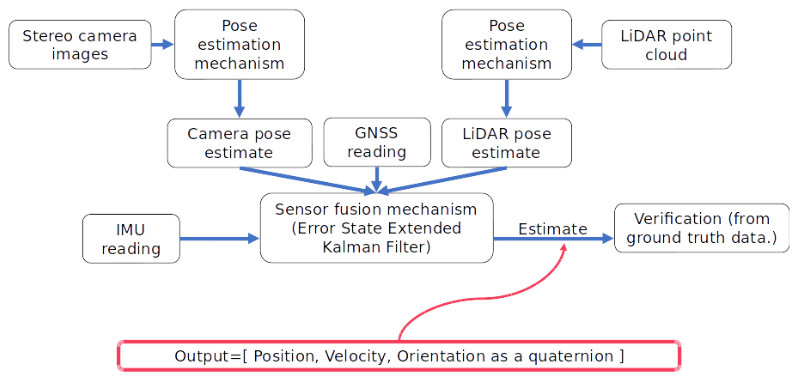
\includegraphics[width=\textwidth]{figs/system-block-diagram.png}
	\end{center}
	\vspace{-0.5cm}
	\caption{System block diagram}
	\label{fig:pa:systemBlockDiagram}
	\vspace{0.5cm}
\end{figure}

The system is implemented on \gls{ROS}, along with evaluation and visualization mechanisms for demonstrating functionality. Main programming language used is Python. Each of the components mentioned in the above discussion will be explained in detail, in the subsequent sections.







%%%%%%%%%%%%%%%
\section{Coordinate frames}
Apart from each sensor's own coordinate frame, in which they provide measurements, we define the following coordinate frames which will be used in the rest of this report.\\\\
\begin{tabular}{p{0.2\linewidth} p{0.75\linewidth} } 
	Inertial frame & An earth fixed right-handed rectilinear coordinate frame with x, y and z axes pointing towards East, North and Up directions respectively (ENU frame). The origin of the frame is determined by the information given in the dataset being used.\\\\
	Body frame & A right-handed rectilinear coordinate frame fixed to the vehicle with x, y and z directions pointing lateral, front and upward directions of the vehicle respectively.
\end{tabular}\\\\
Figure \ref{fig:pa:coordinateFrames} illustrates the above-mentioned coordinate frames.
\begin{figure}[htp]
	\begin{center}
	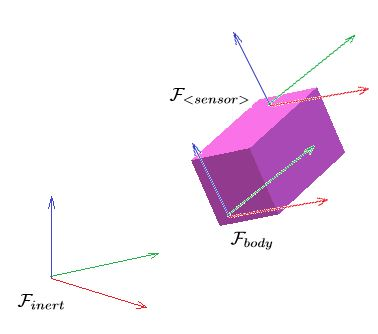
\includegraphics[width=0.6\textwidth]{figs/coordinate-frames.jpg}
	\end{center}
	\vspace{-0.5cm}
	\caption[Coordinate frames]{Illustration of the coordinate frames. x, y and z axes of each coordinate frame is depicted in red, green and blue colours, respectively. The cuboid represents the vehicle. The sensor is assumed to be mounted on the front side of the roof of the vehicle.}
	\label{fig:pa:coordinateFrames}
	\vspace{0.5cm}
\end{figure}






%%%%%%%%%%%%%%%%
\section{Datasets}
We have been using three public datasets, namely, \gls{NCLT} dataset\cite{pa:NCLTDataset}, \gls{KITTI} dataset for tracking\cite{pa:KITTIDataset} and \gls{KAIST} Urban dataset\cite{pa:KAISTDataset}. In addition, we expect to use the EU-Long Term dataset\cite{pa:EULTDataset}. All these datasets include data from sensors that are sufficient for the sensor fusion mechanism, along with ground truth data. Details of the datasets are given in table \ref{table:pa:Datasets}.
% TODO: dataset info table
\begin{table}[htp]
\centering
\begin{tabular}{ |p{0.1\textwidth}|p{0.27\textwidth}|p{0.2\textwidth}|p{0.10\textwidth}|p{0.18\textwidth}|  }
	\hline
	\textbf{Dataset} & \textbf{Sensors} & \textbf{Ground truth} & \textbf{Distance} & \textbf{Data Format}\\
	\hline
	KITTTI  & $1\times$ $64$-layer LiDAR \newline $2\times$ grayscale camera \newline $2\times$ stereo camera \newline $1\times$ GPS-RTK/INS & scene flow, odometry object detection and tracking, road and lane&  $39.2$ km & png (camera) \newline txt(GPA-RTK/INS) \newline bin (LiDAR)\\
	\hline 
	KAIST & $2\times$ $16$-layer LiDAR \newline $2\times$ $1$-layer LiDAR\newline $2\times$ monocular camera\newline $1\times$ consumer-level GPS\newline $1\times$ GPS-RTK\newline $1\times$ fiber optic gyro\newline $1\times$ independant IMU\newline $2\times$ wheel encoder\newline $1\times$ altimeter & SLAM algorithm for vehicle self-localization &$190.989$ km & bin(LiDAR)\newline png(camera)\newline csv(GPS-RTK/IMU)\\
	\hline
	NCLT & $1\times$ $32$-layer LiDAR\newline $2\times$ planar LiDAR\newline $1\times$ camera\newline $1\times$ independant IMU\newline$1\times$ fibre optic gyro\newline $1\times$ consumer-level GPS\newline $1\times$ GPS-RTK\newline & SLAM algorithm for vehicle self-localization with GPS-RTK &$147.4$ km & tiff(image)\newline csv(GPS-RTK/IMU)\newline bin(LiDAR)\\
	\hline
	EU-Long Term & $2\times$ $32$-layer LiDAR\newline $1\times$ $4$-layer LiDAR\newline $1\times$ $1$-layer LiDAR\newline $2\times$ stereo camera \newline $2\times$ fisheye camera\newline $1\times$ radar\newline $1\times$ GPS-RTK\newline $1\times$ independant IMU\newline & GPS-RTK/IMU for vehicle self-localization & $63.4$ km & rosbag (All-in-one)\\
	\hline
\end{tabular}
\caption{Dataset information}
\label{table:pa:Datasets}
\vspace{0.5cm}
\end{table}







%%%%%%%%%%%% ch start %%%%%%%%%%%

\section{Comparison of Bayesian filters}
As mentioned in the introduction, Bayesian filters are the most used sensor fusion mechanism. However, there is a variety of Bayesian filters with their own advantages and disadvantages. Hence, a thorough study was done in-order to select the most suitable Bayesian framework for this problem, which is presented under this section.

Kalman Filters are the most widely used sensor data fusion algorithms. There 
are many extensions to the basic Kalman Filter (which is known as the Linear Kalman Filter), allowing them to be used in variety of applications. Table \ref{table:ch:KalmanFilterComparison} provides a 
comparison between different types of Kalman filters. Note that the computational complexity of the filters increases from left to right.
\begin{table}[htp]
	\centering
	\begin{tabular}{|p{3.4cm}|p{3.4cm}|p{3.4cm}|p{3.4cm}|} 
		\hline
		\textbf{Linear Kalman Filter} & \textbf{Extended Kalman Filter} & \textbf{Error State Extended Kalman Filter} & \textbf{Unscented Kalman Filter} \\
		\hline
		Linear Gaussian model&Non-linear Gaussian model&Non-linear  Gaussian model&Non-linear Gaussian model\\
		\hline
		Best linear unbiased estimator (Blue)&Linearize the nonlinear dynamics using Jacobians (Taylor series)&Linearize the nonlinear 
		dynamics of error using Jacobians (Taylor series)&Calculate sigma points and use Unscented Transform to approximate the PDFs directly\\
		\hline
		Estimates the state & Estimates the state& Estimates the error of the state & Estimates the state\\
		\hline
	\end{tabular}
	\caption{Comparison of different types of Kalman Filters}
	\label{table:ch:KalmanFilterComparison}
	\vspace{0.5cm}
\end{table}

Kalman Filters can only be used for Gaussian models. However, we cannot use the Linear Kalman Filter at all because the localization task is not linear. Assuming that the localization problem is Gaussian, other Kalman Filters can be used to tackle the problem. We selected  \gls{UKF} and \gls{ESKF} to implement in python since those two algorithms have shown the best results among Kalman filters, according to \cite{ch24:st2004comparison},\cite{ch25:madyastha2011extended} and \cite{ch26:wan2000unscented}.

\gls{PF} was recently suggested after \gls{KF}s to process arbitrary inertial sensor characteristics, motion dynamics, and noise distributions. When dealing with non-linear models in motion equations and measurement relations with a non-Gaussian noise assumption, the Kalman Filter methods may lead to non-optimal solutions. However, particle filters provide general solutions to many problems where linearization and Gaussian approximations are intractable \cite{ch27:ababsa2004comparison}. A brief comparison of \gls{PF}s and \gls{KF}s is given in Table \ref{table:ch:KFandPFComparison}.
\begin{table}[htp]
\centering
	\begin{tabular}{|c|c|} 
		\hline
		\textbf{Kalman Filters} & \textbf{Particle Filters} \\
		\hline
		Only for Gaussian models & For both Gaussian and non-Gaussian models\\
		\hline
		Only for linear models& For both linear and non-linear models
		\\
		\hline
		Low computational complexity&High computational complexity\\
		\hline
	\end{tabular}
	\caption{A brief comparison of Kalman Filters and Particle Filters}
	\label{table:ch:KFandPFComparison}
	\vspace{0.5cm}
\end{table}

Three filters (namely, \gls{PF}, \gls{ESKF}, and \gls{UKF}) were implemented in a basic level and, compared using the \gls{NCLT} data set to select the best filter for our application. Afterwards, the performance of the  best filter was improved by increasing the number of elements in the state vector, adding \gls{ZUPT} measurements, and fusing relative measurements (visual and \gls{LiDAR} odometry) etc. The state vector used for the basic filter implementations was
\begin{align}
\label{eq:ch:basicStateVector}
   \textbf{x} &= \left[\begin{matrix}{}\textbf{p}\\\textbf{v}\\\textbf{q}\end{matrix}\right]
\end{align}
where,
\begin{align}
	\textbf{p}&=(p_x,p_y,p_z) \text{ position relative to the inertial frame}\\
	\textbf{v}&=(v_x,v_y,v_z) \text{ velocity relative to the inertial frame}\\
	\textbf{q}&=(q_\omega,q_x,q_y,q_z) \text{ quaternion relative to the inertial frame}.
\end{align}

The \gls{ESKF} estimates the error state directly and uses it as a correction to the nominal state. Number of particles used in the \gls{PF} was 1000. Gaussian random noise was added to the particles before applying the motion model, to increase the diversity of the particles. Systematic Resampling was used to resample particles when needed and squared error function was used as the weight function. Following values were selected for the parameters (as defined in \cite{ch26:wan2000unscented}) of the \gls{UKF};
\begin{align}
	\alpha &= 1 \text{ (determines the spread of sigma points)}\\
	\beta & = 2 \text{ (used to incorporate prior knowledge of the PDF of the state)}\\
	k &= 1 \text{ (a secondary scaling factor, similar to $\alpha$)}.
\end{align}

Based on the results obtained (see section \ref{sec:BayesianFilterComparison}), \gls{ESKF} was selected as the best filter to tackle our problem.


%%%%%%%%%%%% ch end %%%%%%%%%%%%%







%%%%%%%%%%%%%%%
\section{Sensor fusion mechanism}
\subsection{The Error State Extended Kalman Filter}
The \gls{ES-EKF} acts as the component responsible for fusing sensor data. As mentioned in section \ref{sec:SystemArchitecture}, our \gls{ES-EKF} currently has 16 nominal state space variables and 15 error state space variables, grouped into 5 sub-vectors, as listed below;
\begin{align}
    \text{Nominal state vector: }\textbf{x} &= \left[\begin{matrix}{}\textbf{p}\\\textbf{v}\\\textbf{q}\\\boldsymbol{a_b}\\\boldsymbol{\omega_b}\end{matrix}\right]
\end{align}
where
\begin{align}
    \textbf{p} &= (p_x, p_y, p_z) \text{ position relative to the inertial frame} \nonumber \\
    \textbf{v} &= (v_x, v_y, v_z) \text{ velocity relative to the inertial frame} \nonumber \\
    \textbf{q} &= (q_w, q_x, q_y, q_z) \text{ quaternion relative to the inertial frame} \nonumber \\
    \boldsymbol{a_b} &= (a_{bx}, a_{by}, a_{bz}) \text{ acceleration biases of the IMU relative to the body frame} \nonumber \\
    \boldsymbol{\omega_b} &= (\omega_{bx}, \omega_{by}, \omega_{bz}) \text{ angular velocity biases of the IMU relative to the body frame}\nonumber
\end{align}
and
\begin{align}
	\text{Error state vector: }\boldsymbol{\delta}\textbf{x} &= \left[\begin{matrix}{}\boldsymbol{\delta}\textbf{p}\\\boldsymbol{\delta}\textbf{v}\\\boldsymbol{\delta}\boldsymbol{\theta}\\\boldsymbol{\delta}\boldsymbol{a_b}\\\boldsymbol{\delta}\boldsymbol{\omega_b}\end{matrix}\right].
\end{align}
Here, $\boldsymbol{\delta}\textbf{p}, \boldsymbol{\delta}\textbf{v}, \boldsymbol{\delta}\boldsymbol{a_b}$ and $\boldsymbol{\delta}\boldsymbol{\omega_b}$ correspond to the error states of position, velocity, accelerometer bias and gyroscope bias, respectively. $\boldsymbol{\delta}\boldsymbol{\theta}$ is the error in orientation, expressed as an axis-angle vector. Furthermore, $\boldsymbol{\delta}\boldsymbol{a_b}$ and $\boldsymbol{\delta}\boldsymbol{\omega_b}$ are considered as global errors. Relationships used for the prediction step of the filter are given below.\\
Nominal state update:
\begin{align}
    \check{\textbf{p}}_k &= \hat{\textbf{p}}_{k-1}+\hat{\textbf{v}}_{k-1}\Delta t + \frac{1}{2} \left( \textbf{R}_{inert,body}\left(\textbf{a}_{m_{k-1}}-\hat{\textbf{a}}_{b_{k-1}}\right)+\textbf{g}\right)\Delta t^2 \\
    \check{\textbf{v}}_k &= \hat{\textbf{v}}_{k-1}+\left(\textbf{R}_{inert,body}\left(\textbf{a}_{m_{k-1}}-\hat{\textbf{a}}_{b_{k-1}}\right)+\textbf{g}\right)\Delta t \\
    \check{\textbf{q}}_k &= \hat{\textbf{q}}_{k-1}\otimes \textbf{q}\left\{\left(\boldsymbol{\omega}_{m_{k-1}}-\hat{\boldsymbol{\omega}}_{b_{k-1}}\right)\Delta t\right\} \\
    \check{\textbf{a}}_{b_k} &= \hat{\textbf{a}}_{b_{k-1}} \\
    \check{\boldsymbol{\omega}}_{b_{k}} &= \hat{\boldsymbol{\omega}}_{b_{k-1}}
\end{align}
with
\begin{align}
	\textbf{a}_{m_{k}} &= \text{Acceleration measured by accelerometer at k\textsuperscript{th} instance}\\
	\boldsymbol{\omega}_{m_{k}} &= \text{Angular velocity measured by gyroscope at k\textsuperscript{th} instance}\\
    \textbf{R}_{inert,body} &= \text{Rotation matrix corresponding to $\hat{\textbf{q}}_{k-1}$} \\
	\textbf{g} &= \text{Gravity vector w.r.t inertial frame}\\
	\otimes &= \text{Quaternion composition operator.}
\end{align}
Error state covariance matrix update:
\begin{align}
    \Check{\textbf{P}}_k &= \textbf{F}_x\hat{\textbf{P}}_{k-1}\textbf{F}_x^T + \textbf{F}_i\textbf{Q}_i\textbf{F}_i^T
\end{align}
where
\begin{align}
	\textbf{P}_k &= \text{Error state covariance matrix at k\textsuperscript{th} instance}\\
	\textbf{F}_x &= \left.\frac{\partial f}{\partial \boldsymbol{\delta}\textbf{x}}\right|_{\textbf{x}=\hat{\textbf{x}}_{k-1} , \boldsymbol{\delta}\textbf{x}=\textbf{0} , \textbf{w}=\textbf{0}}\\
	\textbf{F}_i &= \left.\frac{\partial f}{\partial \textbf{w}}\right|_{\textbf{x}=\hat{\textbf{x}}_{k-1} , \boldsymbol{\delta}\textbf{x}=\textbf{0} , \textbf{w}=\textbf{0}}\\
	f(.) &= \text{Function representing the motion model}\\
	\textbf{w} &= \text{Process noise vector}\\
	\textbf{Q}_i &= \text{Process noise covariance matrix}.
\end{align}
The equations pertaining to the correction process, upon receiving a measurement update is given below.
\begin{align}
    \textbf{K}_k &= \check{\textbf{P}}_k\textbf{H}^T\left(\textbf{H}\check{\textbf{P}}_k\textbf{H}^T+\textbf{V}\right)^{-1} \\
    \hat{\textbf{P}}_k &= \left(\textbf{I}-\textbf{K}_k\textbf{H}\right)\check{\textbf{P}}_k\\
	\hat{\boldsymbol{\delta}\textbf{x}_k} &= \textbf{K}_k \left(\textbf{y}-h\left(\check{\textbf{x}}_k\right)\right)\\
	\hat{\textbf{x}}_k &= \check{\textbf{x}}_k \oplus \hat{\boldsymbol{\delta}\textbf{x}}_k\\
	\hat{\boldsymbol{\delta}\textbf{x}}_k & \leftarrow \textbf{0}.
\end{align}
Here,
\begin{align}
	h(.) &= \text{Measurement function}\\
	\textbf{H} &= \text{Jacobian of the measurement function, relative to the error state,}\nonumber\\
	&\quad\text{ evaluated at zero}\\
	\textbf{V} &= \text{Measurement noise matrix}\\
	\textbf{y} &= \text{Measurement vector}\\
	\textbf{I} &= \text{Identity matrix of suitable dimension}\\
	\oplus &= \text{Operator representing the combination of nominal state and error state }\nonumber\\
	&\quad\text{ vectors}.
\end{align}
For a detailed explanation of the \gls{ES-EKF}, we refer the reader to \cite{pa:Sola2017QuaternionKinematics}.

\subsection{Stochastic cloning and backward smoothing}
Following the works of Emter et. al\cite{pa:Emter2018StochasticCloning},  we have implemented a stochastic cloning framework along with the \gls{ES-EKF}, as a mean of integrating relative measurements obtained from sensors such as wheel odometer and visual/\gls{LiDAR} odometry algorithms. Since a relative measurement relates the current state of the vehicle to a previous state, it is required to propagate the corrections resultant from absolute measurements to all the previous states as well. In-order to achieve this, a \gls{RTS} backward smoother was integrated.


\subsection{State buffer}
It is essential to store a window of previous estimates obtained as the output of the \gls{ES-EKF}, in-order to be used when fusing a relative measurement, under stochastic cloning framework. A buffer with predefined length was implemented to achieve this functionality. Once a prediction is done by the \gls{ES-EKF}, the estimate is added to the buffer. If the buffer is full, the oldest estimate will be removed, keeping the buffer length a constant.

Other than the estimate itself, the motion model inputs that resulted the prediction of the estimate and the prediction covariance matrix are also stored in this buffer. In addition to the stochastic cloning mechanism, they are used in propagating the effect of an absolute measurement correction across all the states of the buffer.

\subsection{Time synchronization}
Measurements from different sensors arrive at different times, in different rates. These asynchronous arrivals are handled using the \gls{ROS}'s in-built multi-threading behaviour of subscriber callback functions. Each sensor publishes data to its own \gls{ROS} topic, for which the localization module is subscribed to. Hence, each publication will invoke a callback function, which includes the logic for carrying out either a prediction or a correction step, depending on the measurement received.

When an absolute correction is to be carried out, the filter first searches the state buffer, for the state with the closest timestamp to that of the measurement. Then it performs correction steps on that state. After it has been completed, the effect of the correction has to be propagated to all the remaining states in the buffer. States having later timestamps will be adjusted by re-predicting them based on the corrected state. States with earlier timestamps will be adjusted through performing \gls{RTS} smoothing. A similar procedure is carried out upon receiving a relative measurement, except that, backward smoothing with \gls{RTS} smoother will not be performed.

In this manner, a delayed measurement can still contribute to a correction, unless it is too delayed, so that the state corresponding to its timestamp no longer exists in the state buffer.

If a prediction is to be carried out, the filter will only search for the latest timestamp of the states. If it is greater than that of the prediction input, the input will be neglected. Otherwise, a prediction will be carried out and the newly predicted state will be added to the state buffer.

% TODO: add image illustrating time synchronization


\subsection{Zero Velocity Update measurements}
Some of the physical constraints that govern the motion of a vehicle can be incorporated into the sensor fusion mechanism, in-order to make the estimate more accurate. \gls{ZUPT} measurements, generated based on the fact that the motion of a vehicle is constrained only towards its longitudinal direction, is one such constraint that can be employed to couple the positional measurements with the heading estimation \cite{pa:Dissanayake2001ZUPT}. 

However, it should be noted that, the advantages of \gls{ZUPT} measurements come at a cost. Since they are fed into the \gls{ES-EKF} as ordinary absolute measurements, they reduce the estimated covariance of the error, causing the filter to be overconfident on its estimate. Furthermore, once diverged due to erroneous measurements, the estimate takes a longer time to converge back to the ground truth, after starting to receive correct measurements. These effects should be balanced out by carefully tuning the noise variance of the \gls{ZUPT} measurement.






%%%%%%%%%%%%%%%% ra start %%%%%%%%%%%%%%%%%%

\section{Visual Odometry}
Out of the sensors that we use for localization process, cameras are the cheapest. However, they are capable of providing rich information of the environment, which allows us to recognize the environment robustly and accurately. Therefore, camera based visual odometry \gls{SLAM} solutions are becoming very popular, and can be used in our system as a solution for \gls{GNSS} outages. 

\subsection{System Selection}
\label{subsec:vodomSystemSelection}
Monocular camera based systems are the most commonly used for visual odometry because of the low cost and the smaller sensor setup. However, estimations are not reliable and inaccurate because depth cannot be calculated using one camera \cite{ra:ORB_SLAM2}. Therefore, stereo camera based systems were selected as the best solution for our system. As implementation of this algorithm was not within the project scope, we had to find a solution with an existing implementation. Following criteria were used when selecting a suitable method:
\begin{itemize}
    \item Should not depend on previously generated feature maps
    \item Should provide real time output
    \item Accuracy
    \item Availability of proper implementation
\end{itemize}

\gls{ORBSLAM} \cite{ra:ORB_SLAM2} and \gls{S-PTAM} \cite{ra:S-PTAM} were the best solutions available. Furthermore, they had proper implementations, available for free. Comparing the results they have obtained by testing these algorithms using the KITTI dataset \cite{ra:KITTI}, \gls{ORBSLAM} showed superior perfomance over \gls{S-PTAM}. Furthermore, the implementation of the \gls{ORBSLAM} algorithm was fairly detailed. Hence, we selected \gls{ORBSLAM} as the best solution.


\subsection{ORB SLAM 2 algorithm}
This is an extension of the previously implemented \gls{ORBSLAM} algorithm \cite{ra:ORB_SLAM}, which was only for the monocular systems. In the \gls{ORBSLAM}, they have extended the previous implementation for the stereo cameras with accuracy improvements\cite{ra:ORB_SLAM2}. 
\begin{figure}[t]
	\centering
	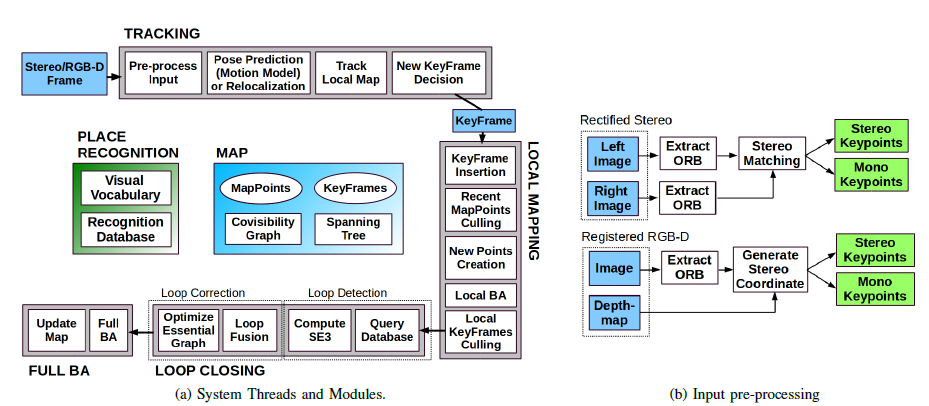
\includegraphics[width=\textwidth]{figs/ORB_SYSTEM.png}
	\vspace{-0.5cm}
	\caption[ORB SLAM 2 architecture]{ORB SLAM 2 architecture \cite{ra:ORB_SLAM2}}
	\label{fig:ra:ORB_SYSTEM}
	\vspace{0.5cm}
\end{figure}

Pre-processing architecture is shown in figure \ref{fig:ra:ORB_SYSTEM}(b). Features of the rectified stereo images will be extracted using the ORB feature extractor \cite{ra:ORB} and extracted features will be matched with the previous frame to identify the stereo key points. 

General view of the system architecture is shown in figure \ref{fig:ra:ORB_SYSTEM}(a). System is consisted of three main parallel threads, namely;
\begin{enumerate}
	\item the Tracking thread to localize the camera with every frame by finding feature matches to the local map and minimizing the re-projection error applying motion-only \gls{BA}
	\item the Local Mapping thread to manage the local map and optimize it, performing local BA\gls{BA}
	\item the Loop Closing thread to detect large loops and correct the accumulated drift by performing a pose-graph optimization \cite{ra:ORB_SLAM2}.
\end{enumerate} 

In the existing code, the vehicle is localized on a local map created using the feature points. However, for our system, we needed to get the relative transform of the vehicle, between two stereo frames. Hence, we modified the existing algorithm to receive relative transform of the vehicle, directly, as the output. The result is published as a \gls{ROS} message.

\gls{ORBSLAM} has been designed and setup only for the \gls{KITTI} and \gls{TUM} datasets. We added the image rectification functionality for the \gls{KAIST}, as we will be using that dataset for our testing purposes.

One drawback of the \gls{ORBSLAM} algorithm is the absence of a reliability metric (eg: estimated variance of the error) for the estimate. In order to circumvent this problem, we have been testing different methods to obtain an error covarince matrix. One of the methods tested was to estimate covariance values based on the number of features matched between each pair of frames. We hypothesized that the error should be reduced if a higher number of features have been detected. However, this hypothesis has been observed to be invalid (see section \ref{sec:VisualOdometry}). Hence, alternatives are being sought to overcome this issue. 

%%%%%%%%%%%%%%%% ra end %%%%%%%%%%%%%%%%%%%%








%%%%%%%%%%%%%%%% hi start %%%%%%%%%%%%%%%%%%


\section{Lidar Odometry}
In vehicle localization, out of the sensors that we use, \gls{LiDAR} is the most expensive and accurate sensor. It is capable of providing point clouds of the surrounding environment (well-defined rich information) which allows us to recognize the environment robustly and accurately. 360-degree feature space exploration is the best advantage that we can gain from a high-end \gls{LiDAR}, which we can’t obtain with cameras and other sensors regardless of their quality. However, this elevated accuracy comes at a significantly higher cost, relative to the rest of the sensors.

\subsection{Method Selection}
As implementation of a \gls{LiDAR} odometry algorithm is not within the scope of this project, we had to find a solution with an existing implementation. The criteria followed in this selection was similar to that as in the case of visual odometry algorithm (see section \ref{subsec:vodomSystemSelection}). Few alternatives that could be used in this respect are listed in table \ref{table:ha:DifferentLOdomMethods}.
\begin{table}[htp]
	\centering
	\begin{tabular}{|p{0.3\textwidth}|p{0.3\textwidth}|p{0.15\textwidth}|p{0.15\textwidth}|} 
		\hline
		\textbf{Algorithm} & \textbf{Features} & \textbf{Complexity} & \textbf{Robustness} \\
		\hline
		Conventional \gls{ICP}&Accuracy mainly depends on the correspondence
		matching&Low&Low\\
		\hline
		\gls{NDT}&No correspondence feature matching&Moderate&Moderate\\
		\hline
		\gls{LOAM}&IMU data makes estimation more robust& High & High\\
		\hline
		\gls{LeGO-LOAM}&IMU data makes estimation more robust& High & Very High\\
		\hline
	\end{tabular}
	\caption{Different LiDAR odometry algorithms}
	\label{table:ha:DifferentLOdomMethods}
	\vspace{0.5cm}
\end{table}

\gls{LOAM} \cite{hi:LOAM} and \gls{LeGO-LOAM} \cite{hi:LeGO-LOAM} were the best solutions that we found with a proper implementation. Comparing the benchmark errors received by testing the algorithms using the \gls{KITTI} dataset, \gls{LeGO-LOAM} showed the better estimation. Depending on the results, along with the comparison presented in table \ref{table:ha:DifferentLOdomMethods}, we selected \gls{LeGO-LOAM} as the best solution for our localization module.

\subsection{Lego-LOAM}
\gls{LeGO-LOAM} algorithm is an extension of the \gls{LOAM} algorithm with new features added to make it more accurate, robust and fast in terms of computation. Following list presents some such modifications.
\begin{itemize}
    \item Project the \gls{LiDAR} points into a range image 
    \item Segment the ground plane and separate the ground plane from the image
    \item Apply image based segmentation method (clustering) to extract separate clusters
    \item Feature extraction phase is more robust and fast since feature extraction is carried out with segmented objects and planes, rather than raw points, as in \gls{LOAM}.
\end{itemize}

\begin{figure}[t]
	\centering
	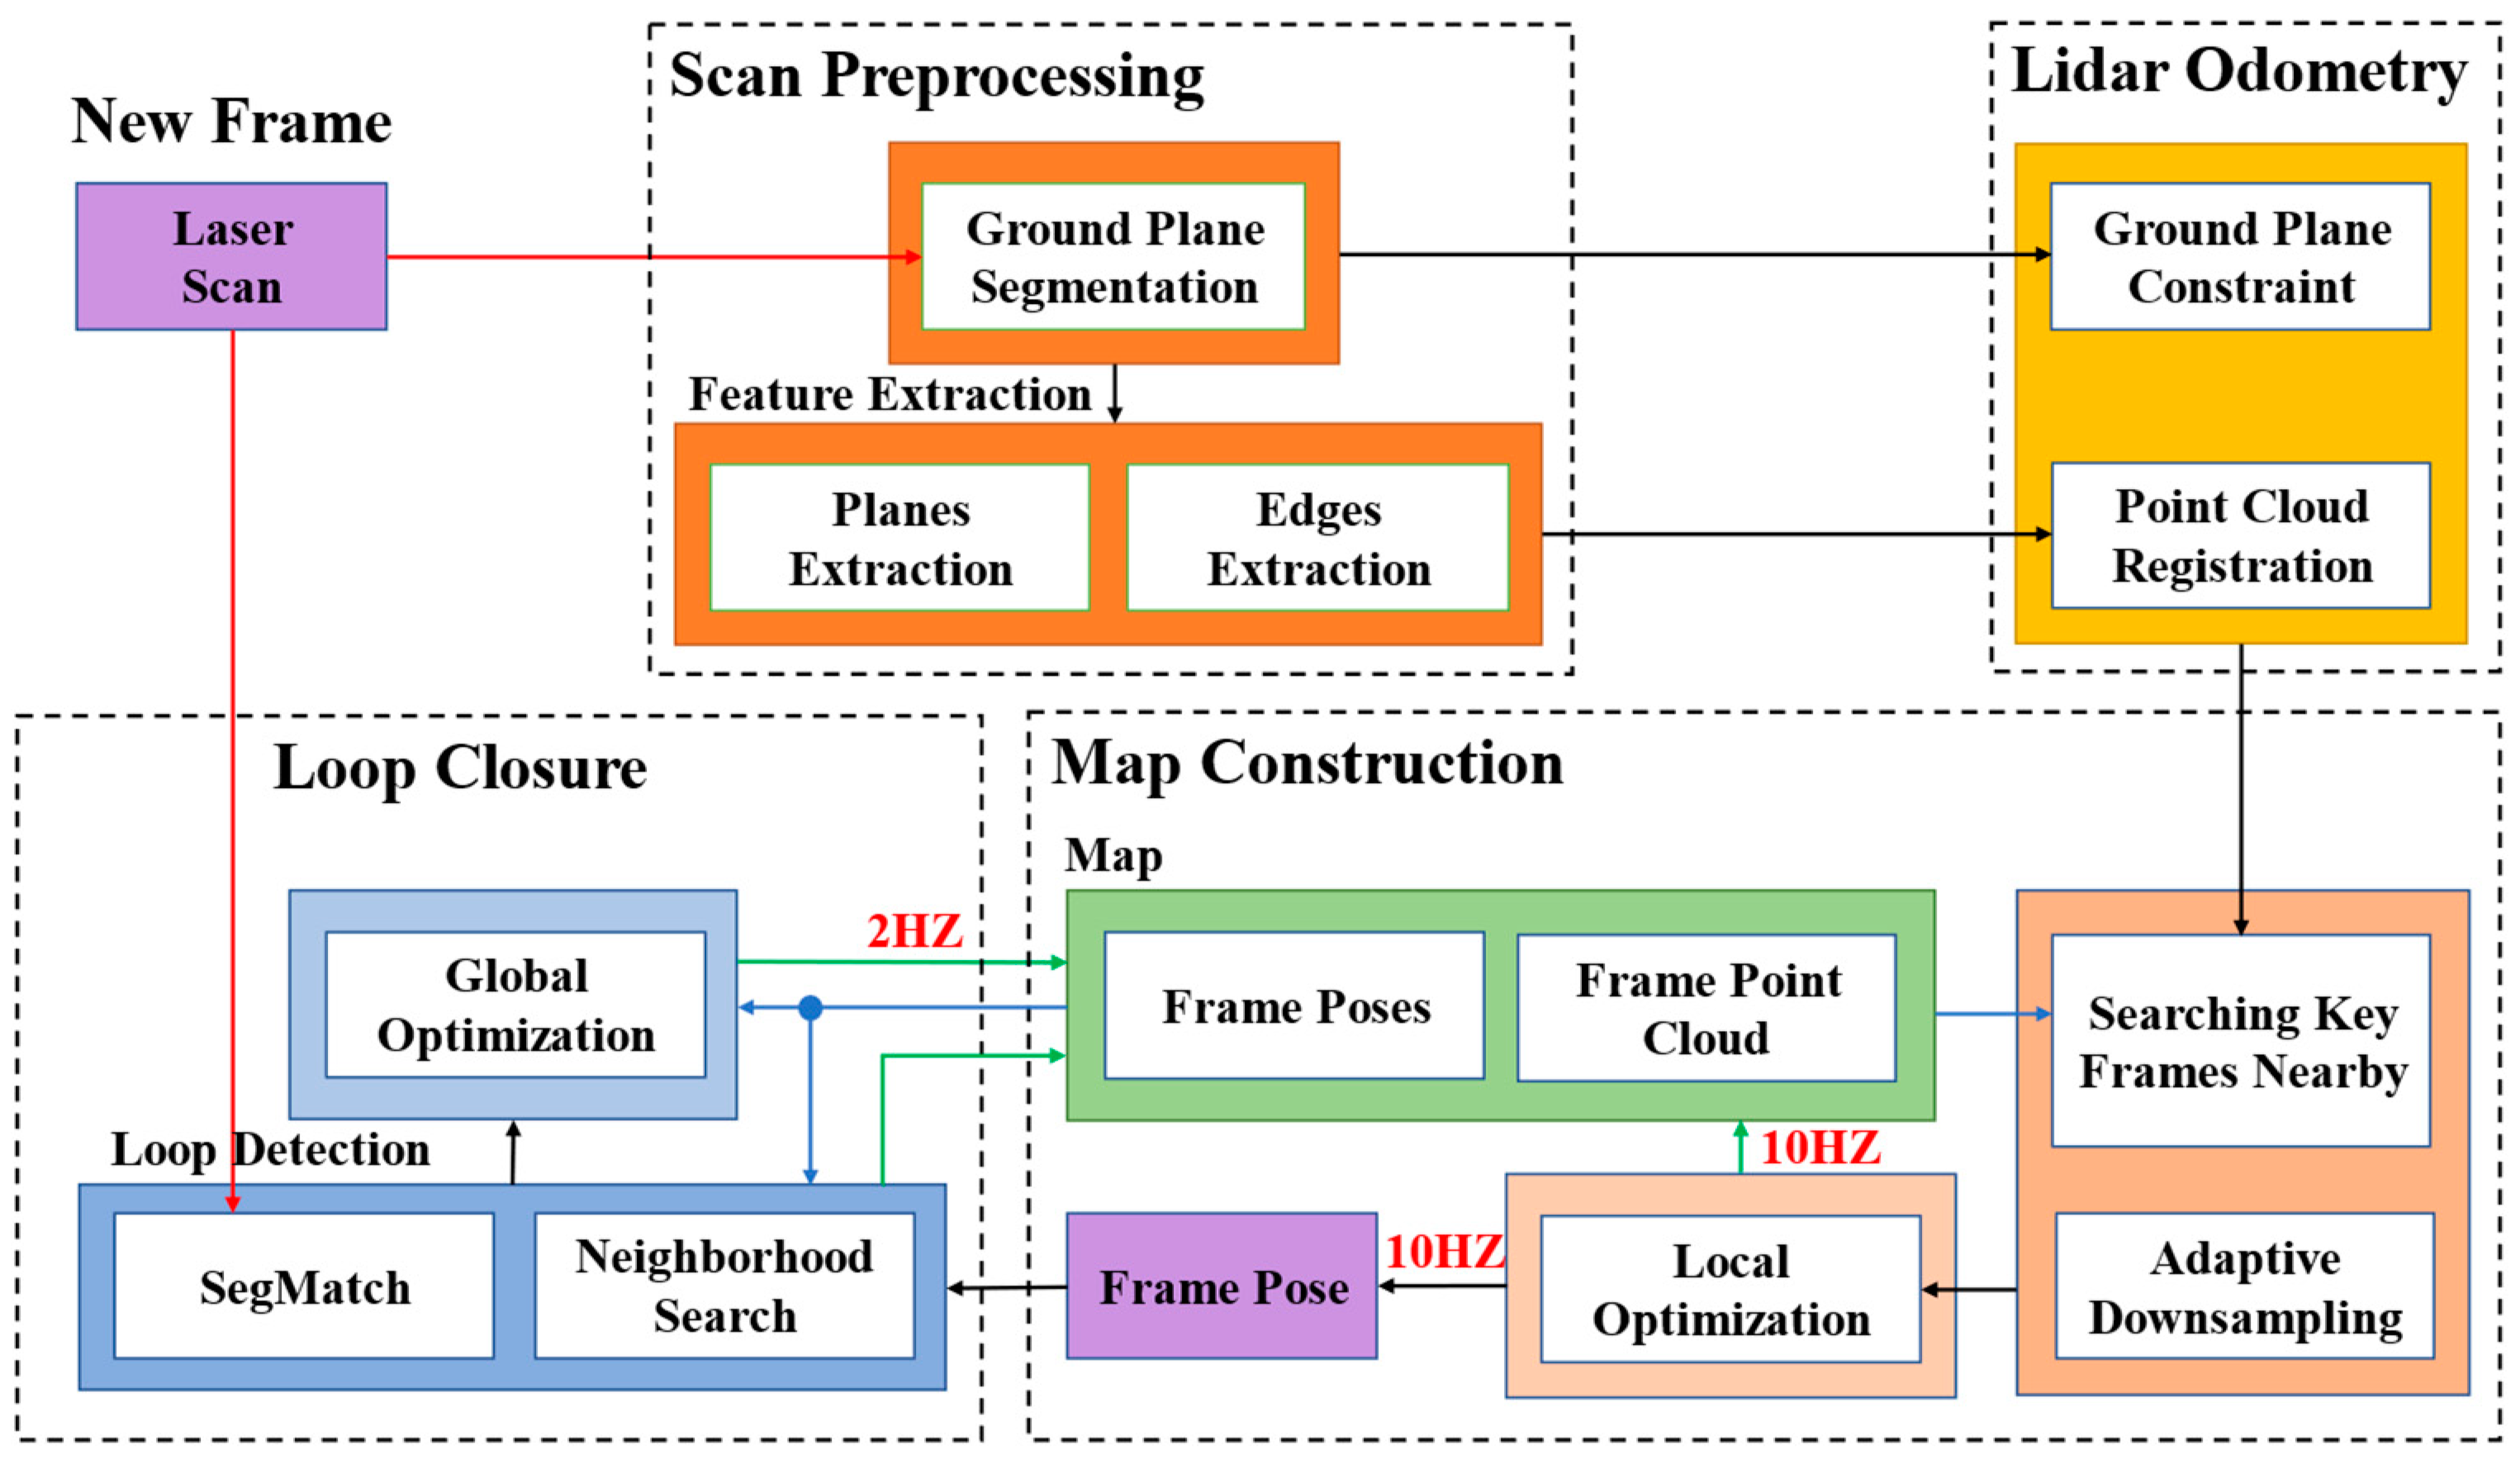
\includegraphics[ width=\textwidth]{figs/loam_architect.png}
	\vspace{-0.5cm}
	\caption[Lego-LOAM system architecture]{Lego-LOAM system architecture\cite{hi:LeGO-LOAM}}
	\label{fig:hi:LeGO_LOAM_SYSTEM}
	\vspace{0.5cm}
\end{figure}

General view of the \gls{LeGO-LOAM} system architecture is shown in figure \ref{fig:hi:LeGO_LOAM_SYSTEM}. System consists of four main modules; scan preprocessing, odometry, map construction and global optimization. Scan preprocessing module projects the \gls{LiDAR} points onto a range image, segments the ground plane and separate the ground plane from the image. Then it applies image based segmentation methods for ground plane segmentation and edge features  are extracted from the projected image. Odometry module takes care of feature matching and transformation optimization for \gls{LiDAR} point cloud registration and generates odometry measurement. Map construction module uses the previous key frames and odometry estimation to construct the map and also adds fast optimization to the odometry estimation. Loop closure module adds global optimization and drift correction to the map and makes the construction much more drift free.

In the existing code, the vehicle is localized on a local map created using the map construction module. However, for our system, we need to get the relative transform of the vehicle as an output. Therefore, the adjustments have been made to the existing algorithm to receive relative transform of the vehicle between every \gls{LiDAR} scan.

The issue of not having a mechanism to obtain the covariance of the pose-estimate error is a limitation of this algorithm, as well. Hence, we expect to find solutions for this issue based on metrics such as the final optimized error in \gls{LM} algorithm \cite{hi:LM_optimization} etc.


%%%%%%%%%%%%%%%% hi end %%%%%%%%%%%%%%%%%%%%










%%%%%%%%%%%%%%%%
\section{Implementation on Robot Operating System}
The system was implemented on \gls{ROS}, targetting the easy integration with other modules (path planning, perception etc.) of the autonomous vehicle. Furthermore, the \gls{ROS} environment facilitates the following;
\begin{itemize}
	\item Visualizing results (through Rviz, Multiplot etc.)
	\item In-built multi-threading for handling asynchronous data feeds
	\item Controlling simulation time
	\item Inter-process communication through \gls{ROS} topics
	\item Debugging (using tools such as Node Graphs, TF Tree etc.)
	\item Handling transformations (through TF)
\end{itemize}
Apart from the nodes for visual and \gls{LiDAR} odometry algorithms, the system consists of 3 main nodes, namely, the Data Feeder, Locator and the Evaluator. Each of these nodes will be described separately, in the following sub-sections. Figure \ref{fig:pa:nodeGraph} shows the Node Graph obtained for the system.

\begin{figure}[htp]
	\begin{center}
	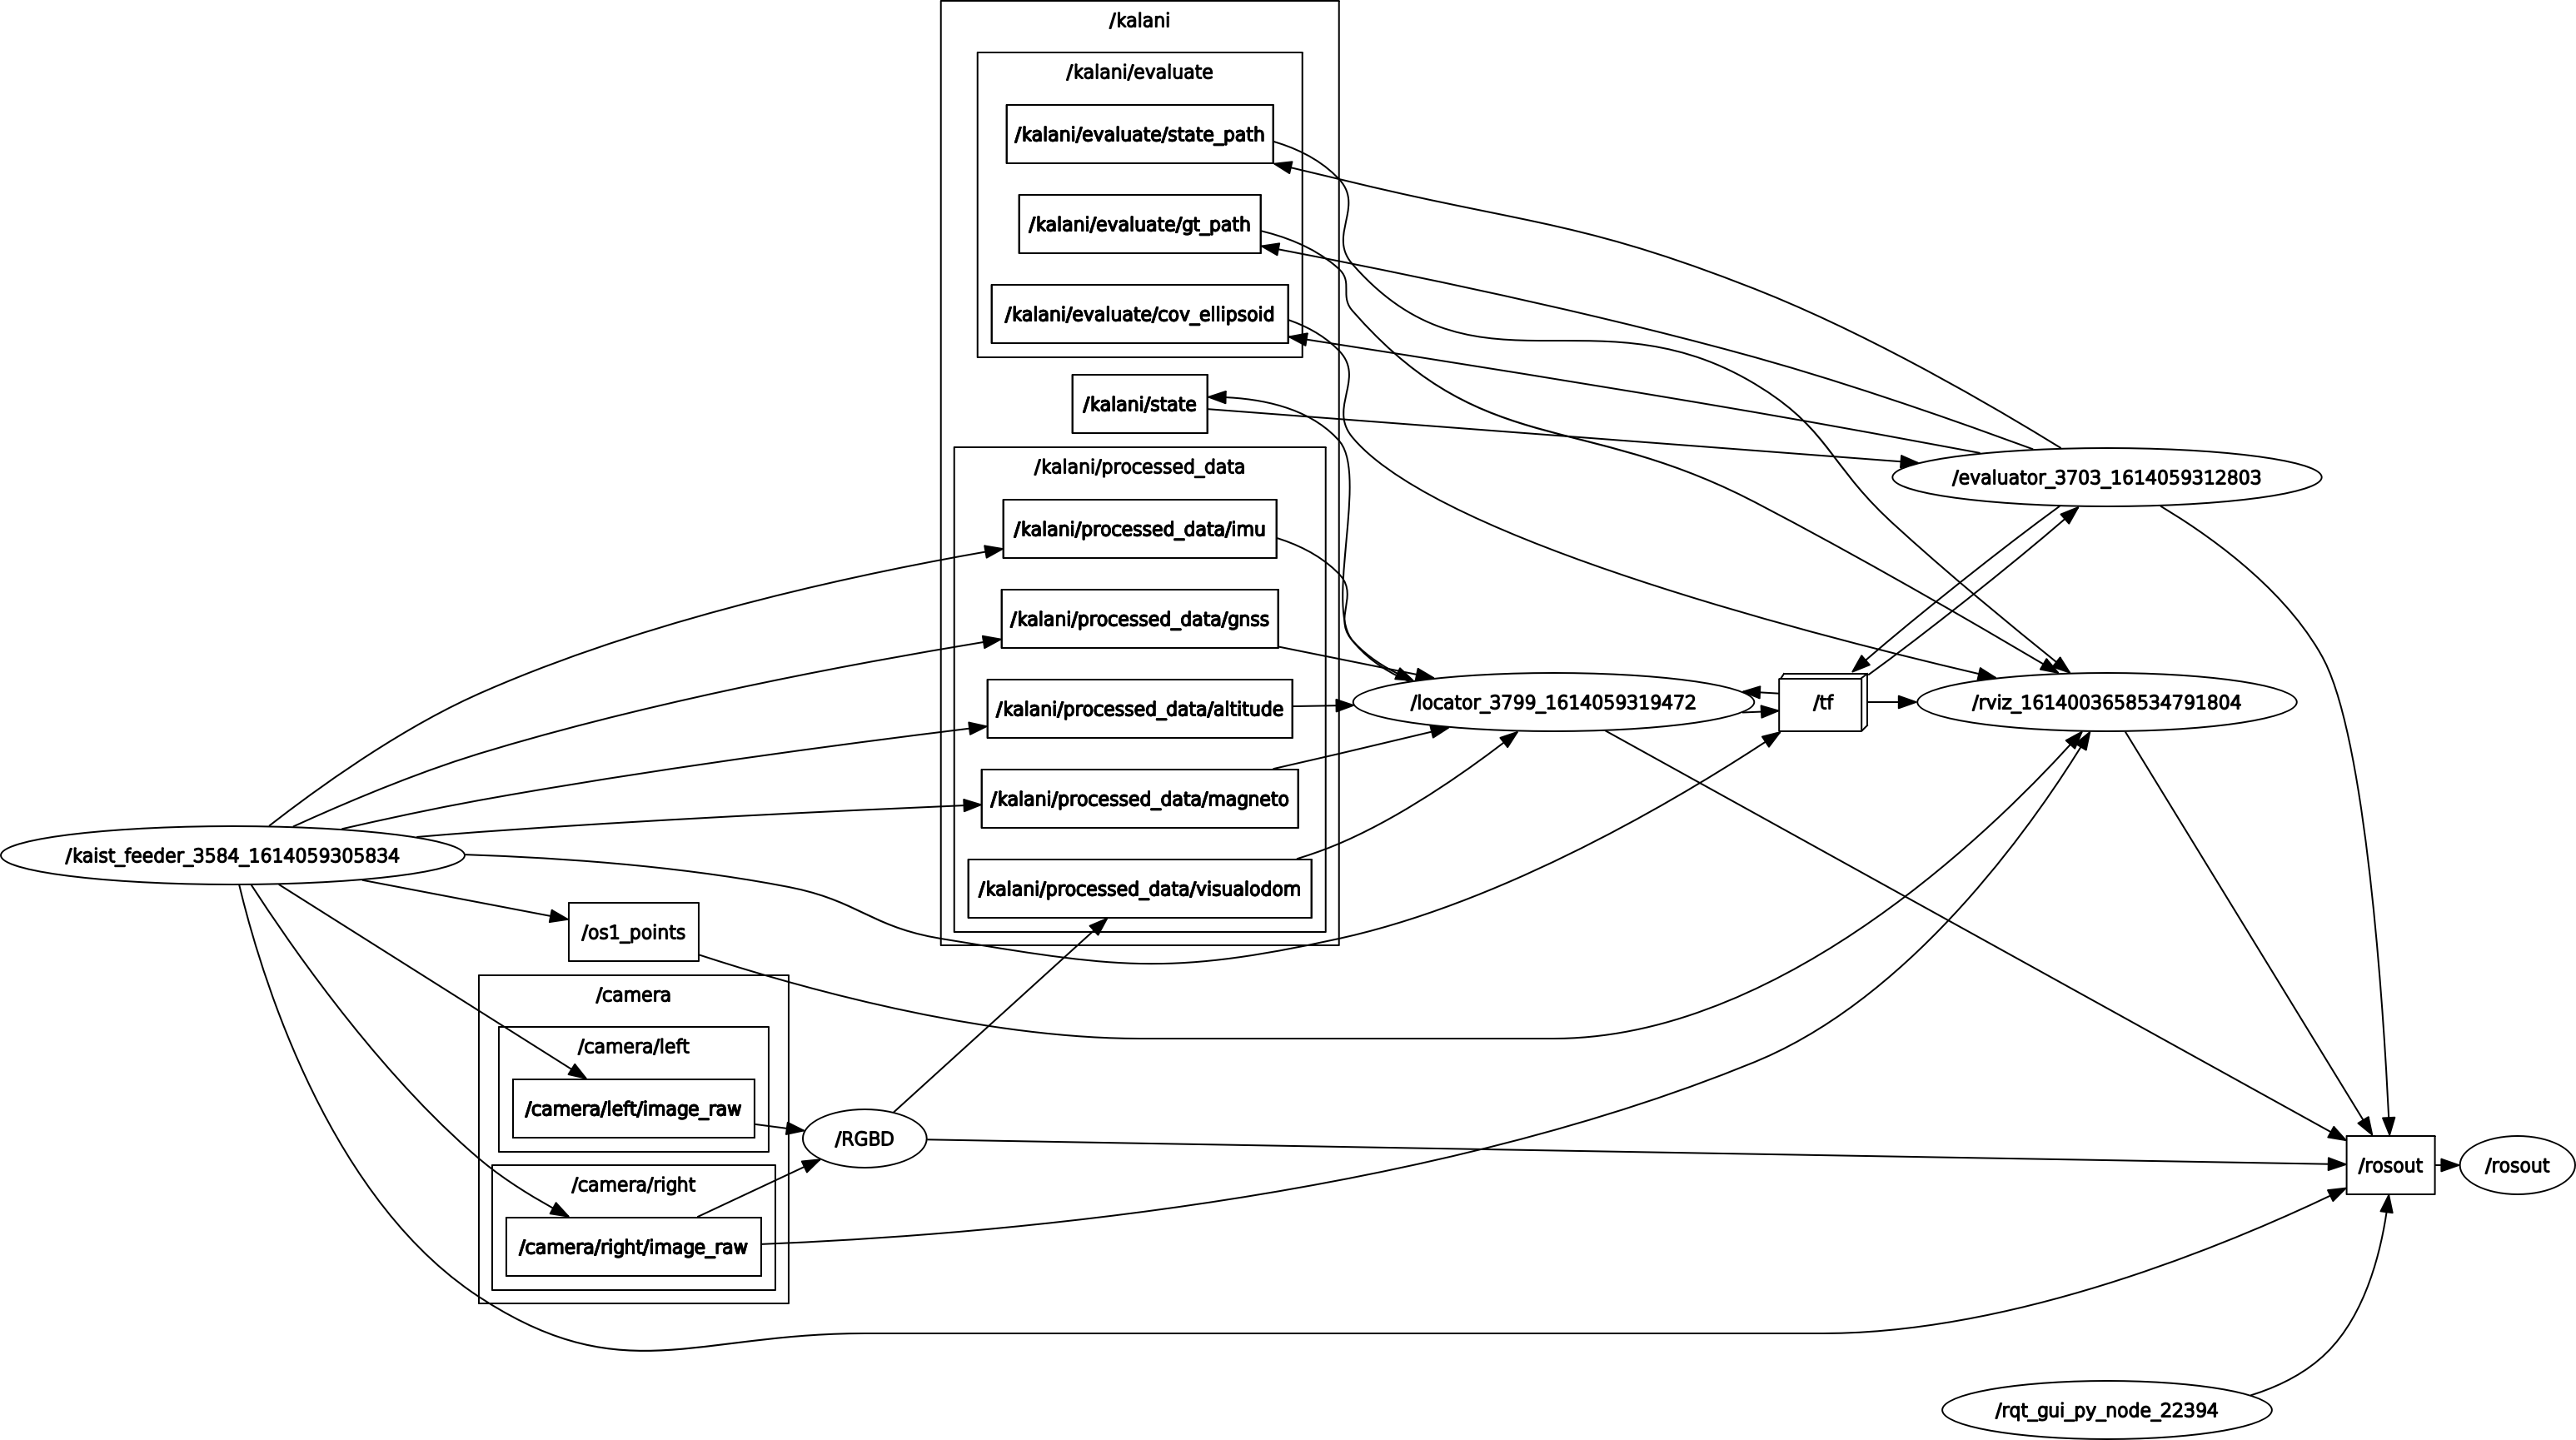
\includegraphics[width=\textwidth]{figs/rosgraph.png}
	\end{center}
	\vspace{-0.5cm}
	\caption[ROS Node Graph]{ROS Node Graph}
	\label{fig:pa:nodeGraph}
	\vspace{0.5cm}
\end{figure}

\subsection{Data Feeder}
This \gls{ROS} node is responsible for publishing sensor data obtained from the dataset, into pre-defined \gls{ROS} topics. Furthermore, it is capable of controlling the simulation clock, so that the simulation timescale can be adjusted. It carries out all the data conversions required (Eg: \gls{GNSS} sensor data need to be converted from \gls{WGS} 84 to the local inertial frame) and publishes the data according to the rates specified by the specifications of the corresponding sensor. Each dataset in use requires a separate Data Feeder, tailored to suit its data format specifications.

\subsection{Locator}
This is the node that is responsible for invoking prediction and correction functions of the \gls{ES-EKF}, upon receiving data from the Data Feeder. Once a prediction is done, it publishes the latest state estimate both as a TF frame update as well as a \gls{ROS} message under a pre-defined topic. The structure of the \gls{ES-EKF} (including state variables, motion model and its Jacobians) is defined within this node, along with the measurement matrices for both absolute and relative measurement updates.

\subsection{Evaluator}
Purpose of this node is to calculate and publish the errors and error confidence bounds (3$\sigma$ bounds) for the state estimate. In addition, it publishes the errors caused in the \gls{GNSS} and magnetometer measurements, with respect to the ground truth. These errors can be visualized on either Rviz or Multiplot tools. Furthermore, it keeps a history of the paths of the estimate and the ground truth, which is also can be visualized on Rviz.




  \chapter{Results}
\label{chapter:results}
\gls{NCLT} dataset was used for the comparison of different filters. Functionality of each component has been tested with \gls{KITTI}, \gls{KAIST} and \gls{NCLT} datasets.



%%%%%%%%% ch start %%%%%%%

\section{Comparison of Bayesian filters}
\label{sec:BayesianFilterComparison}
Data from the \gls{NCLT} dataset has been used for this comparison and the results shown in the discussion have been obtained using sequence 2013.01.10.
\subsection{Performance of translation estimation}
Overall performances (\gls{RMS} error) of all the filters are better than the raw \gls{GNSS} measurements. \gls{UKF} has given the worst estimation while \gls{PF} and \gls{ESKF} have given better results. Table \ref{table:ch:RMSErrorPosition} shows a summary of the results.
\begin{table}[h]
    \centering
    \begin{tabular}{|p{2.5cm}|p{2.5cm}|p{2.5cm}|p{2.5cm}|p{2.5cm}|} 
        \hline
        \textbf{Method} & \textbf{x} & \textbf{y} & \textbf{z}& \textbf{Overall} \\
        \textbf{} & \textbf{direction(m)} & \textbf{direction(m)} & \textbf{direction(m)}& \textbf{position(m)} \\
        \hline
        GPS&6.3278 &9.8746 &5.6387& 13.0133\\
        \hline
        ESKF &4.6824& 2.8655 &7.0109 &8.9044\\
        \hline
        UKF &4.7371& 2.7663 &11.2554 &12.5211
        \\
        \hline
        PF& 4.4488& 2.8587& 6.8126& 8.6242
        \\
        \hline
    \end{tabular}
\caption{Translational \gls{RMS} errors for different Bayesian filters}
\label{table:ch:RMSErrorPosition}
\end{table}

Even though \gls{PF} has given the most accurate results, as shown in figures \ref{fig:ch:errorX} to \ref{fig:ch:errorPositionOverall}, output of the filter is not smooth. Furthermore, the estimate rapidly diverges upon receiving erroneous \gls{GNSS} measurements (see figure \ref{fig:ch:errorPositionOverall}). Adding random samples or increasing the size of the particle set are alternatives for this problem. However, both of these solutions will increase the computational complexity. If both \gls{RMS} error and smoothness are considered, \gls{ESKF} gives the best solution. Z-direction has shown the worst error in all the three filters resulting a large overall positional error. This behaviour is a result of the large error in the altitude measurement, obtained by the \gls{GNSS} receiver. It can be mitigated by using an Altimeter (which is only present in the \gls{KAIST} dataset, out of the three datasets being used).

\begin{figure}[h]
    \centering
    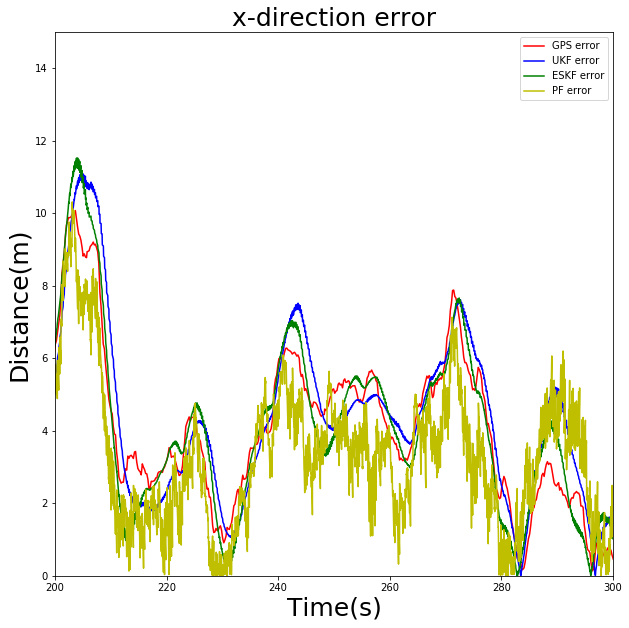
\includegraphics[width=0.7\textwidth]{figs/x_direction.png}
    \caption{Filter comparison - error in x direction}
    \label{fig:ch:errorX}
\end{figure}
\begin{figure}[h]
    \centering
    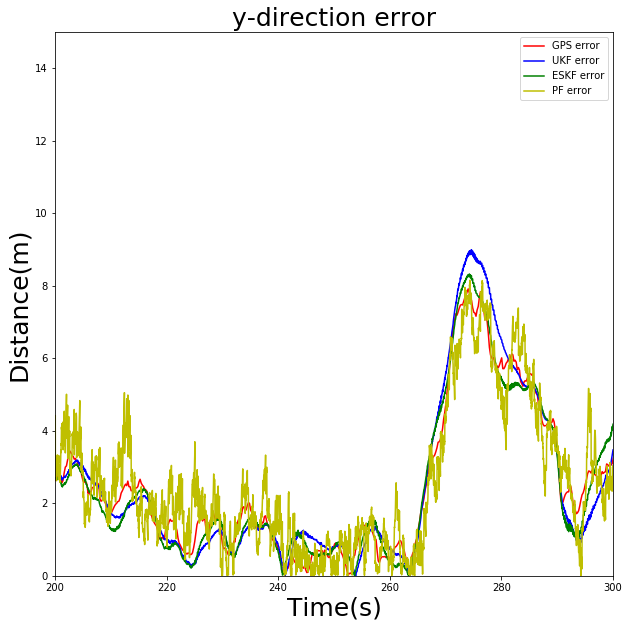
\includegraphics[width=0.7\textwidth]{figs/y_direction.png}
    \caption{Filter comparison - error in y direction}
    \label{fig:ch:errorY}
\end{figure}
\begin{figure}[h]
    \centering
    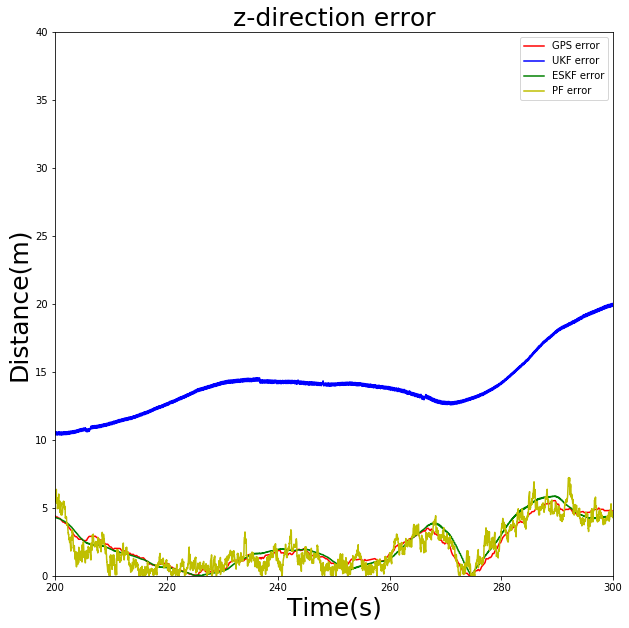
\includegraphics[width=0.7\textwidth]{figs/z_direction.png}
    \caption{Filter comparison - error in z direction}
    \label{fig:ch:errorZ}
\end{figure}
\begin{figure}[h]
    \begin{subfigure}{0.5\textwidth}
        \centering
        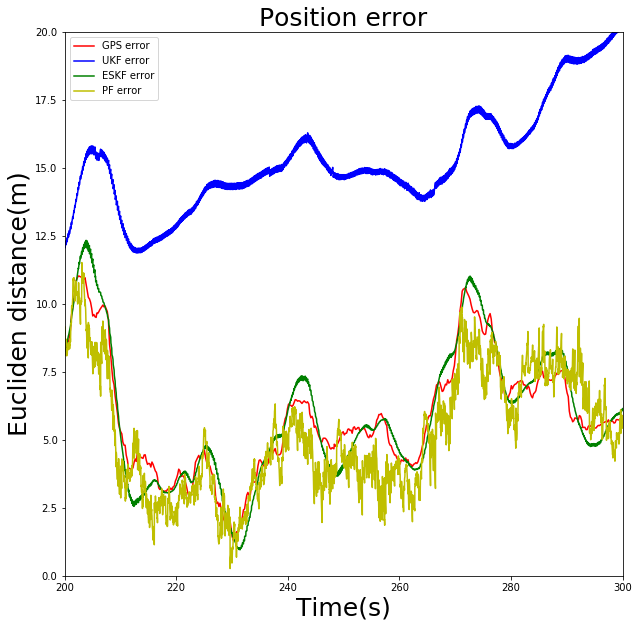
\includegraphics[width=1\textwidth]{figs/overall.png}
        \caption{Excluding the diverged \gls{PF} result}
    \end{subfigure}%
    \begin{subfigure}{0.5\textwidth}
        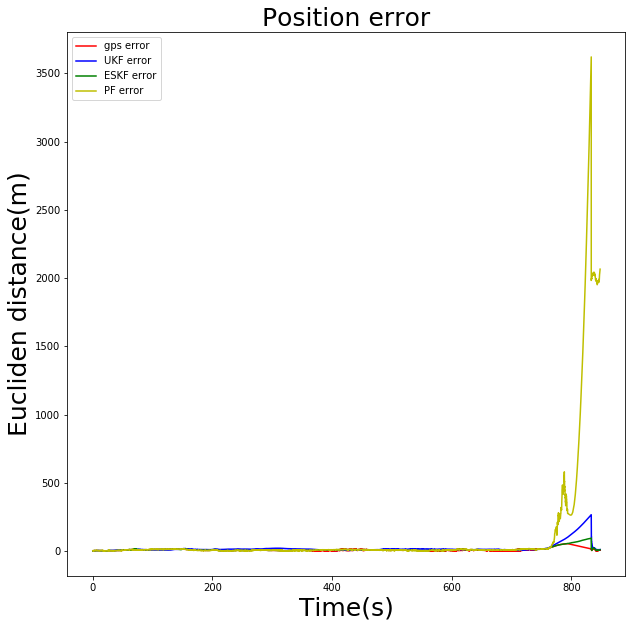
\includegraphics[width=1\textwidth]{figs/overall_diverge.png}
        \caption{Including the diverged \gls{PF} result}
    \end{subfigure}
    \caption{Filter comparison - overall translational error}
    \label{fig:ch:errorPositionOverall}
\end{figure}


\subsection{Performance of orientation estimation}
Raw orientation measurement obtained using the \gls{IMU} + Magnetometer is better than the estimates of all the three filters (see table \ref{table:ch:RMSErrorRotation}). This is due to the noise in the angular velocity measurement, which is confirmed from the reduction of the error when the angular measurement noise variance parameter is increased. \gls{PF} has given the worst estimation. Results of the other two filters are somewhat similar. However, \gls{UKF} has given the best
estimation. Error plots are shown in figures \ref{fig:ch:errorRoll}, \ref{fig:ch:errorPitch} and \ref{fig:ch:errorYaw}.
\begin{table}[h]
    \centering
    \begin{tabular}{|p{4cm}|p{3cm}|p{3cm}|p{3cm}|} 
        \hline
        \textbf{Method} & \textbf{Roll (deg)} & \textbf{Pitch (deg)} & \textbf{Yaw (deg)} \\
        \hline
        \gls{IMU}+Magnetometer & 1.1555 &1.7171 &7.7622\\
        \hline
        ESKF& 2.8258& 3.3362& 8.8584\\
        \hline
        UKF &1.7216& 1.8304& 8.6043
        \\
        \hline
        PF &14.76759& 12.32548 &37.5694
        \\
        \hline
    \end{tabular}
    \caption{Rotational \gls{RMS} errors of different Bayesian filters}
    \label{table:ch:RMSErrorRotation}
\end{table}

\begin{figure}[h]
\centering
	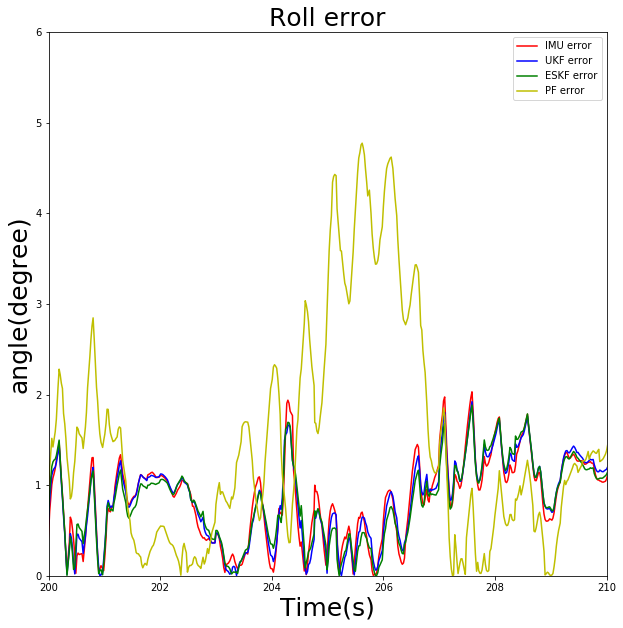
\includegraphics[width=0.7\textwidth]{figs/roll.png}
	\caption{Filter comparison - error in roll}
	\label{fig:ch:errorRoll}
\end{figure}

\begin{figure}[h]
\centering
	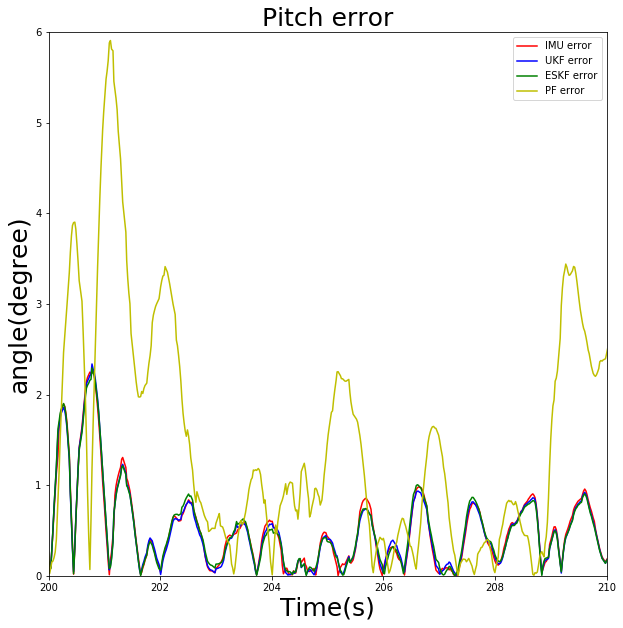
\includegraphics[width=0.7\textwidth]{figs/pitch.png}
	\caption{Filter comparison - error in pitch}
	\label{fig:ch:errorPitch}
\end{figure}

\begin{figure}[h]
\centering
	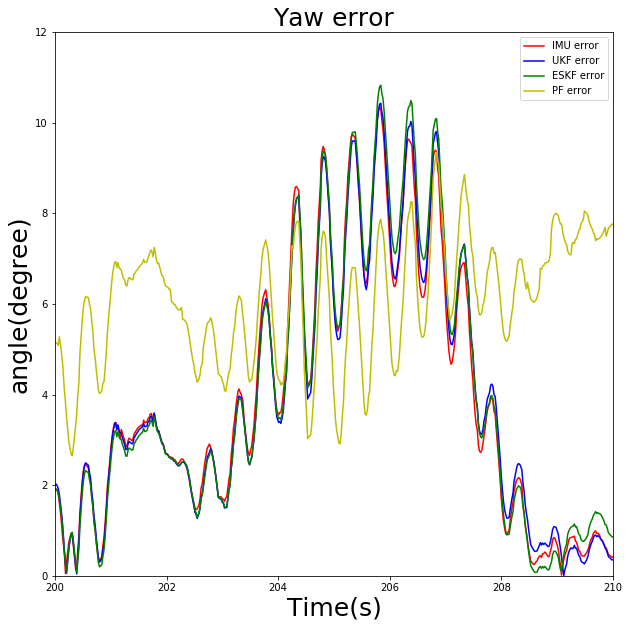
\includegraphics[width=0.7\textwidth]{figs/yaw.png}
	\caption{Filter comparison - error in yaw}
	\label{fig:ch:errorYaw}
\end{figure}


%%%%%%%% ch end %%%%%%%%%





%%%%%%%%%%%%%%%
\section{Sensor fusion mechanism}
The effect of fusing relative measurements through stochastic cloning was observed using the \gls{NCLT} dataset. \gls{GNSS} and Magnetometer data were used as absolute measurements and wheel odometry data were used as relative measurements. A 30 s \gls{GNSS} outage was simulated, and the error in the estimate was observed for the two instances; with and without fusing relative measurements. It was observed that with the integration of relative measurement data, the error remained bounded (see figure \ref{fig:pa:relativeMeasurements}).
\begin{figure}[h]
	\centering
    \begin{subfigure}{\textwidth}
        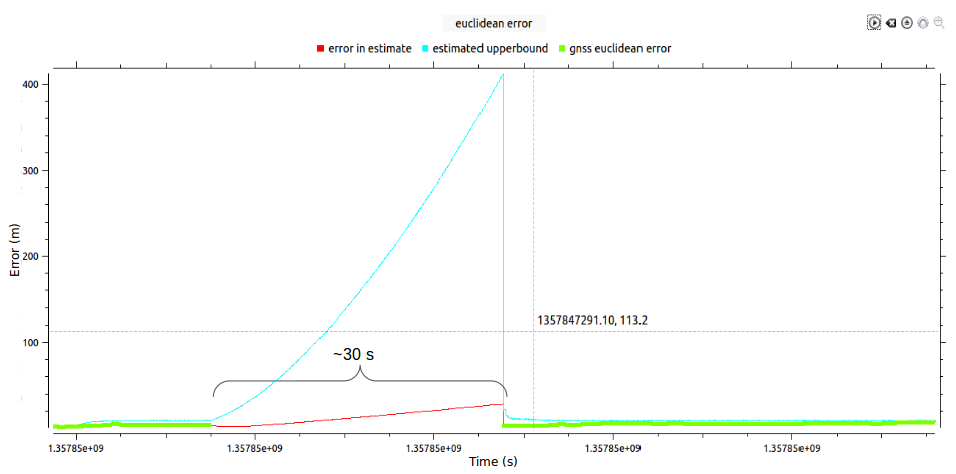
\includegraphics[width=\textwidth]{figs/euclidean-error-wo-rm.png}
        \caption{Euclidean error without relative measurements}
    \end{subfigure}
    \begin{subfigure}{\textwidth}
        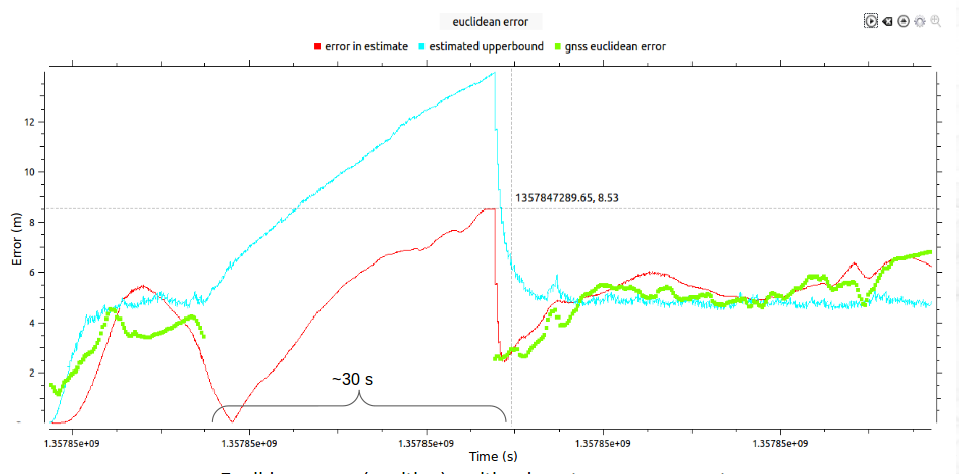
\includegraphics[width=\textwidth]{figs/euclidean-error-with-rm.png}
        \caption{Euclidean error with relative measurements}
    \end{subfigure}
    \caption[Effect of relative measurements]{Effect of relative measurements during a \gls{GNSS} interruption. Green: error in \gls{GNSS} measurements, Red: error in estimate, Cyan: estimated upper bound for the error.}
    \label{fig:pa:relativeMeasurements}
\end{figure}

Adding \gls{ZUPT} measurements has a significant effect on the accuracy of the yaw estimate, as seen from figure \ref{fig:pa:zuptYaw}. When \gls{ZUPT} measurements are applied, the yaw estimate error remains within the estimated error bounds (3$\sigma$ bounds), despite the fact that the magnetometer-estimated yaw is biased.
\begin{figure}[h]
	\centering
    \begin{subfigure}{\textwidth}
        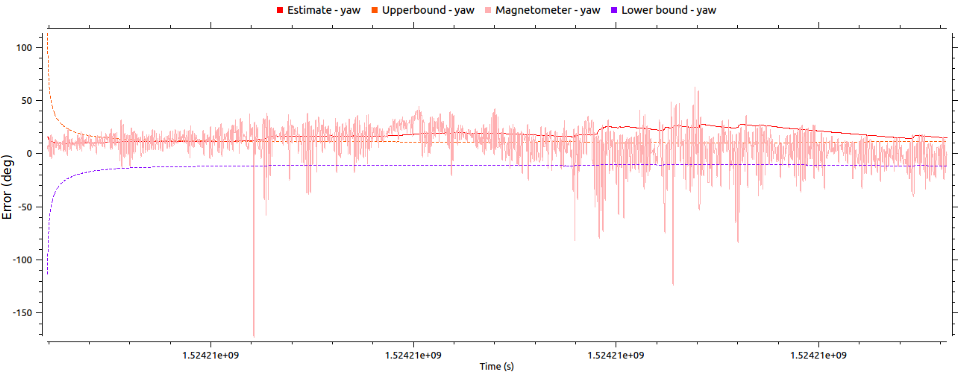
\includegraphics[width=\textwidth]{figs/yaw-without-zupt.png}
        \caption{Yaw estimate without \gls{ZUPT} measurements}
    \end{subfigure}
    \begin{subfigure}{\textwidth}
        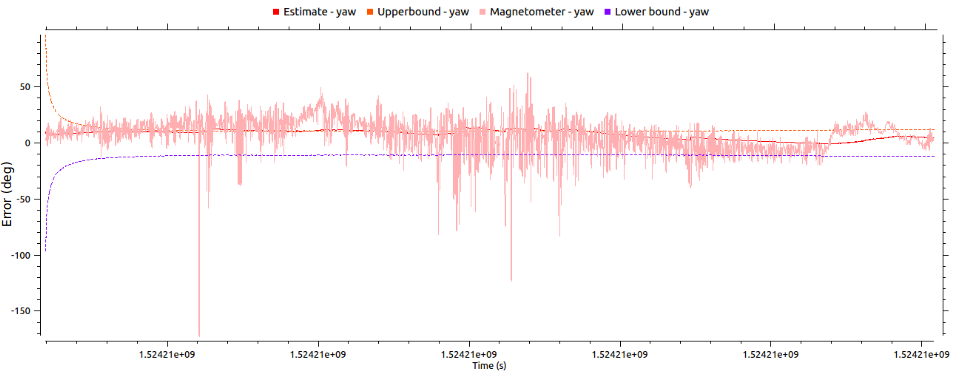
\includegraphics[width=\textwidth]{figs/yaw-with-zupt.png}
        \caption{Yaw estimate with \gls{ZUPT} measurements}
    \end{subfigure}
    \caption[Effect of \gls{ZUPT} measurements on the yaw estimate]{Effect of \gls{ZUPT} measurements on the yaw estimate. Pink: Magnetometer estimated yaw, Red: Filter output, Orange (dashed): Estimated upper bound of the error, Violet (dashed): Estimated lower bound of the error.}
    \label{fig:pa:zuptYaw}
\end{figure}







%%%%%%%%%%%% ra start %%%%%%%%%%%%%%%%%%%%

\section{Visual Odometry}
\label{sec:VisualOdometry}

Experiments were conducted using the \gls{KITTI} and \gls{KAIST} datasets on the \gls{ORBSLAM}. Images in the \gls{KITTI} odometry dataset are rectified images and the ones in the \gls{KAIST} dataset are non-rectified. Therefore, images should be rectified in system for the \gls{KAIST} dataset. Results in the subsequent discussion have been obtained using the \gls{KITTI} dataset. Coordinate axes, x, y and z refer to the coordinate axes of the initial camera frame (Coordinate frame of the camera, when the vehicle started moving).

When running \gls{ORBSLAM} algorithm, it creates a feature points map using the detected feature points (see figure \ref{fig:ra:detected_features}) and localize the vehicle in the feature map. Figure \ref{fig:ra:point_map} shows the estimated path of the vehicle in the map.
\begin{figure}[h]
	\centering
	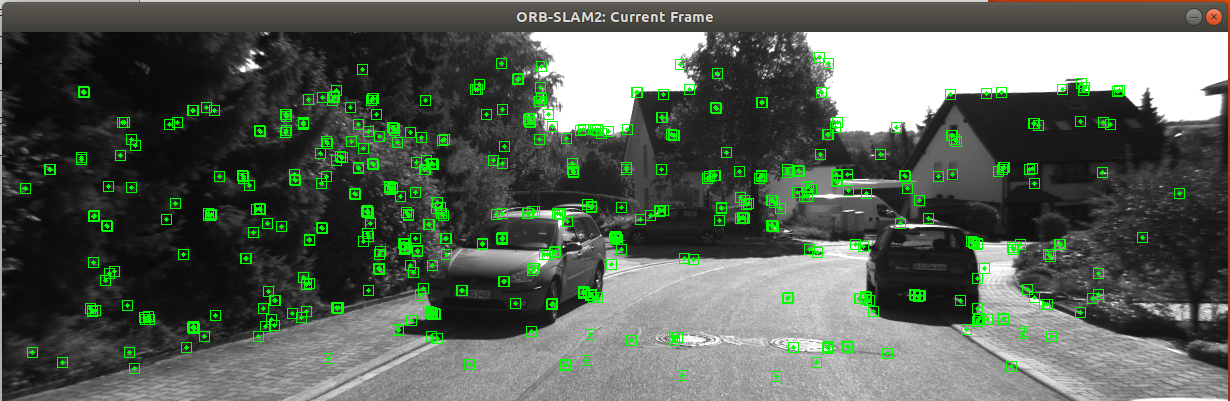
\includegraphics[width=\textwidth]{figs/detected_features.png}
	\vspace{-0.5cm}
	\caption[Detected feature points]{Feature points detected in a frame of \gls{KITTI} sequence 09 when running \gls{ORBSLAM}. Green colour squares indicate the feature points.}
	\label{fig:ra:detected_features}
	\vspace{0.5cm}
\end{figure}
\begin{figure}[h]
	\centering
	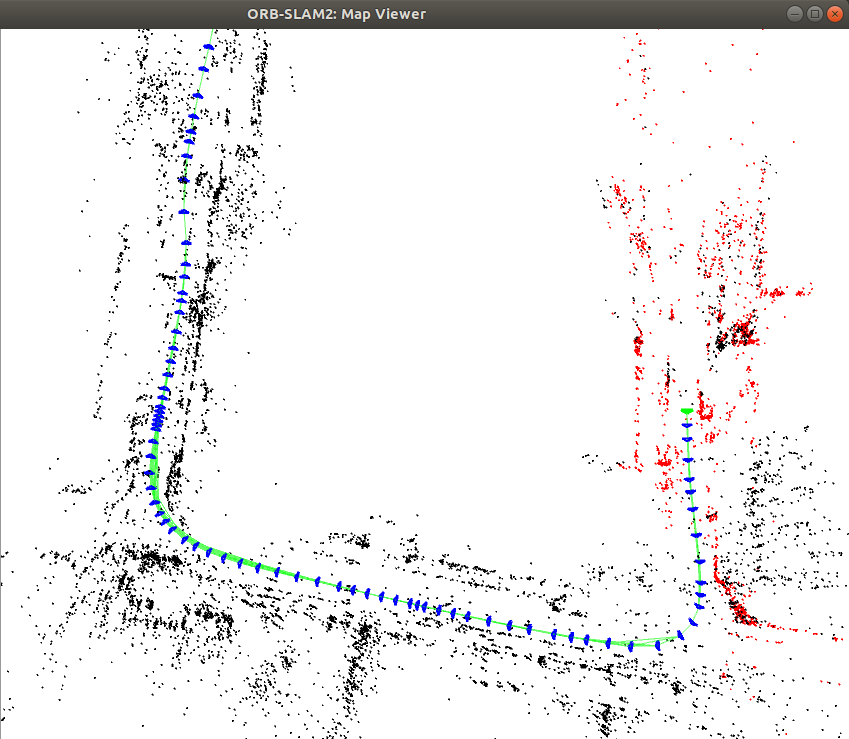
\includegraphics[width=\textwidth]{figs/path_pred.png}
	\vspace{-0.5cm}
	\caption[Map of feature points]{Part of the feature point map generated from \gls{ORBSLAM}, using \gls{KITTI} sequence 00. Estimated path of the vehicle is shown in green colour. Blue triangles show the pose of the camera, in the respective frames.}
	\label{fig:ra:point_map}
	\vspace{0.5cm}
\end{figure}

Figure \ref{fig:ra:xyz_error} shows the position error in the directions of x, y and z with the frame index, and figure \ref{fig:ra:rpy_error} shows the error in the orientation (roll, pitch and yaw) with the frame index. It can be observed that the total position error in a given direction increase with time due to the accumulation of the relative position errors in the estimate.
\begin{figure}[h]
	\centering
	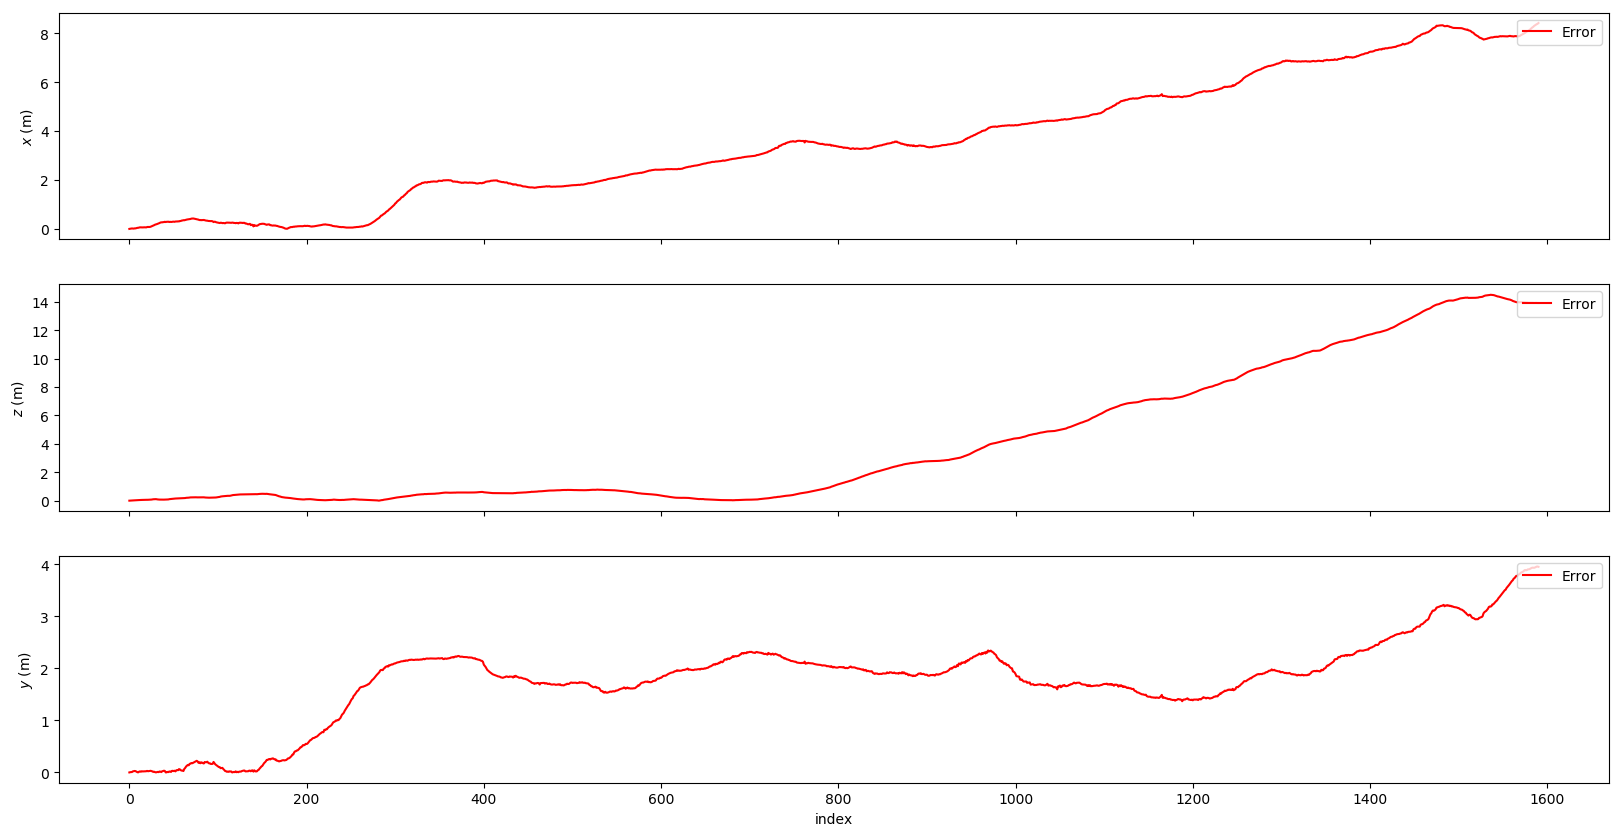
\includegraphics[ width=\textwidth]{figs/xyz_error.png}
	\vspace{-0.5cm}
	\caption[Positional error of \gls{ORBSLAM}]{Positional error of \gls{ORBSLAM} (\gls{KITTI} sequence 09)}
	\label{fig:ra:xyz_error}
	\vspace{0.5cm}
\end{figure}
\begin{figure}[h]
	\centering
	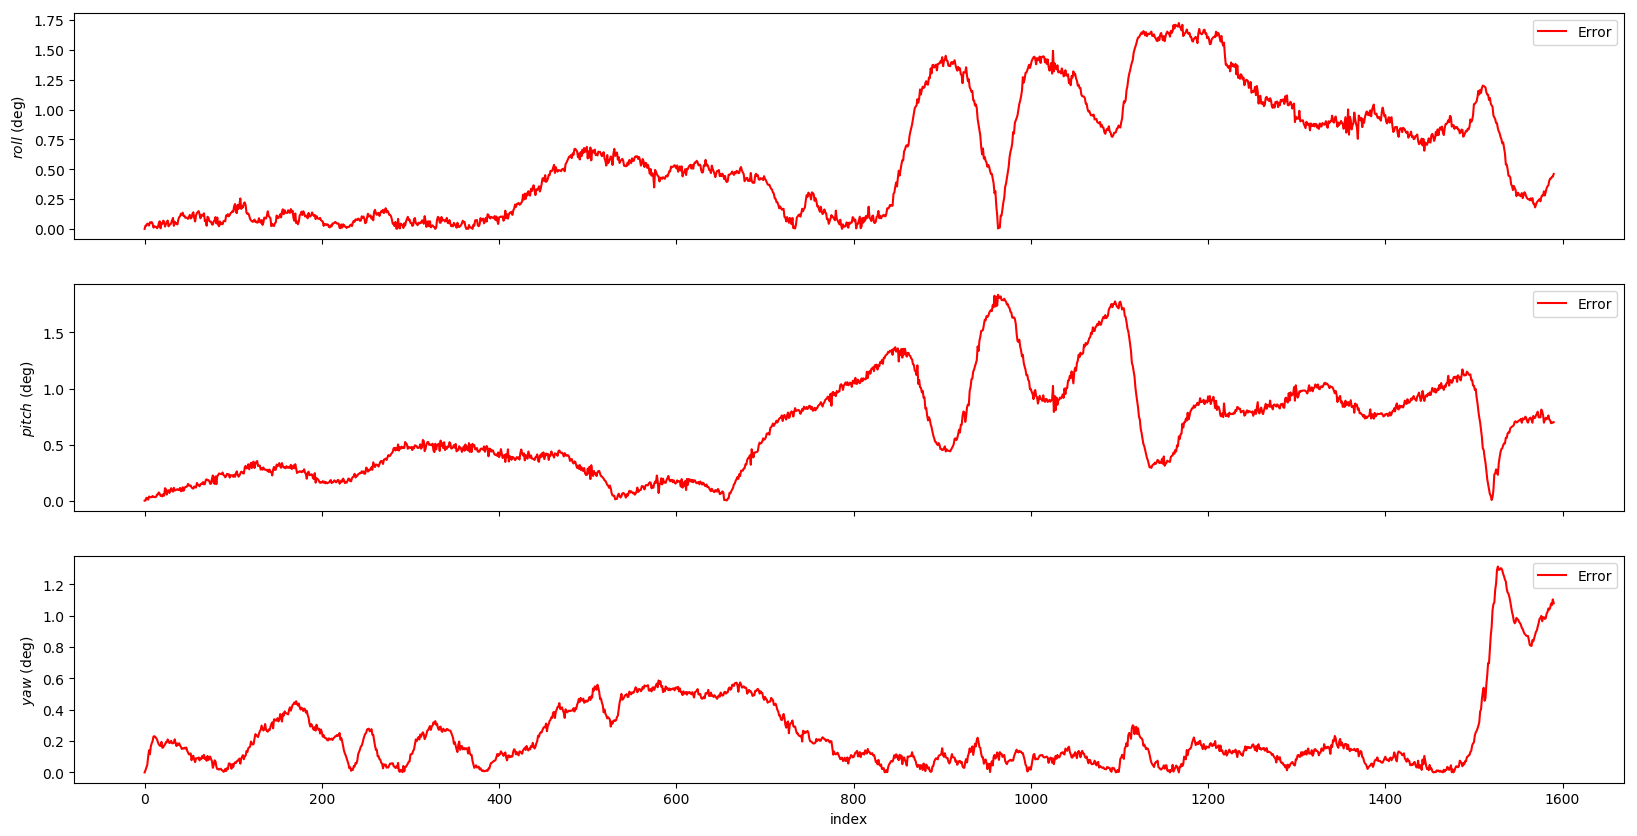
\includegraphics[ width=\textwidth]{figs/rpy_error.png}
	\vspace{-0.5cm}
	\caption[Rotational error of \gls{ORBSLAM}]{Rotational error of \gls{ORBSLAM} (\gls{KITTI} sequence 09)}
	\label{fig:ra:rpy_error}
	\vspace{0.5cm}
\end{figure}

In-order to test the effect of error accumulation, we subtracted the error of the previous frame, from the total error of the current frame, thereby removing the effect of accumulated error, for each frame. This revealed that the error in the relative position/orientation estimate of the algorithm is extremely low (within $\pm$0.1 m for position and $\pm0.2^o$ for orientation, for \gls{KITTI} dataset), which is desirable when using the output as a relative measurement in the fusion mechanism (see figures \ref{fig:ra:xyz_error_allred} and \ref{fig:ra:rpy_error_allred}).
\begin{figure}[h]
	\centering
	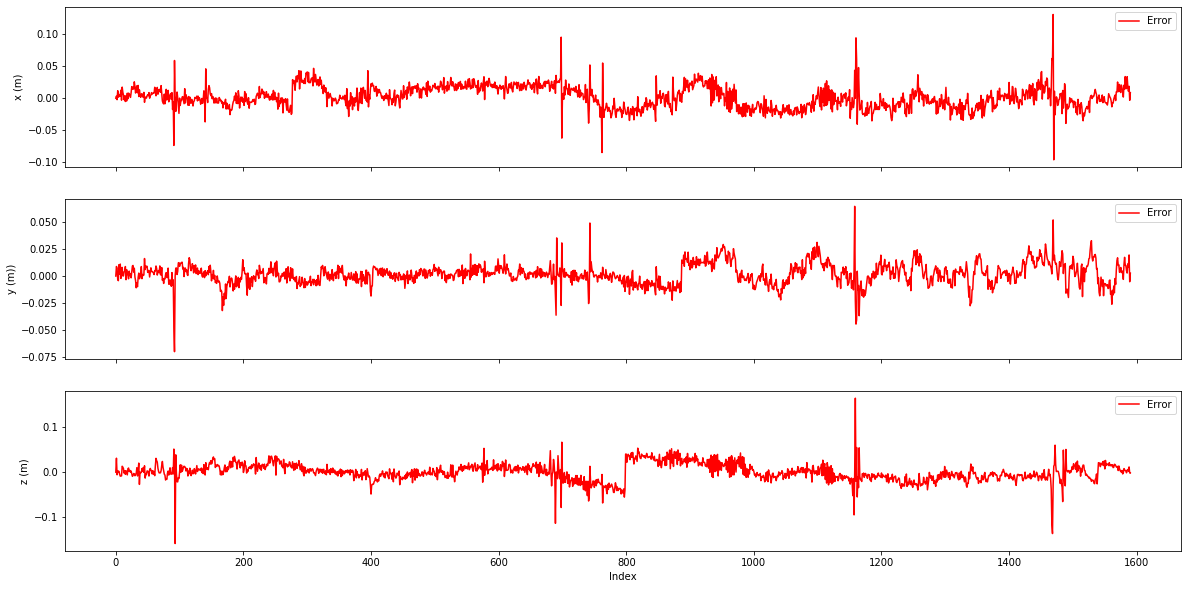
\includegraphics[width=\textwidth]{figs/xyz_error_allred.png}
	\vspace{-0.5cm}
	\caption{Positional error of \gls{ORBSLAM}, after removing the effect of error accumulation}
	\label{fig:ra:xyz_error_allred}
	\vspace{0.5cm}
\end{figure}
\begin{figure}[h]
	\centering
	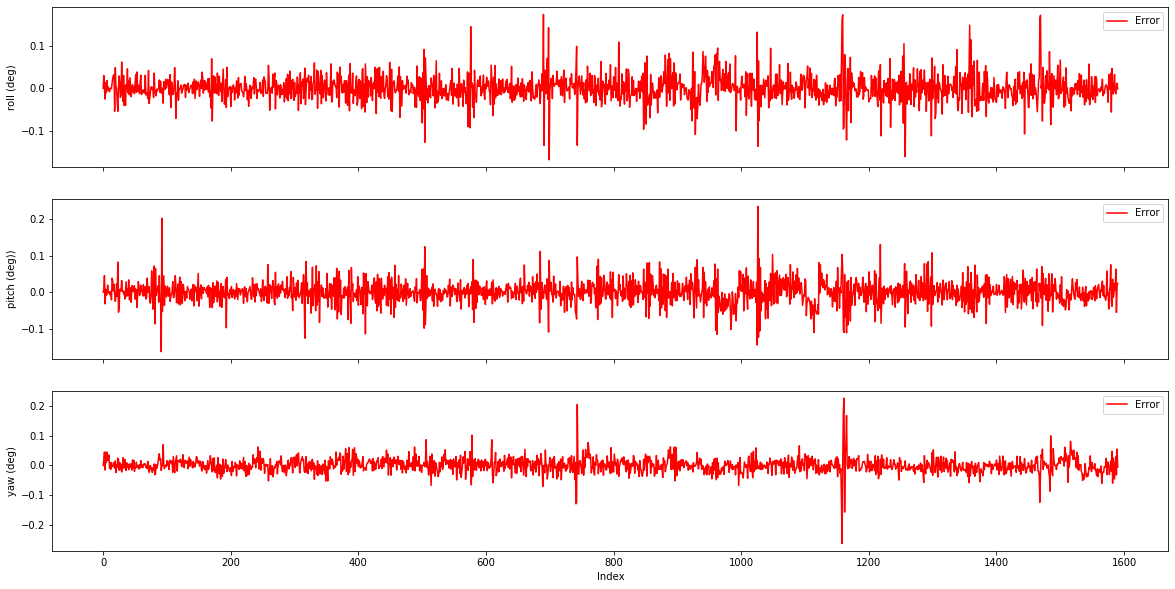
\includegraphics[ width=\textwidth]{figs/rpy_error_allred.png}
	\vspace{-0.5cm}
	\caption{Rotational error of \gls{ORBSLAM}, after removing the effect of error accumulation}
	\label{fig:ra:rpy_error_allred}
	\vspace{0.5cm}
\end{figure}

With the intention of obtaining insights for implementing an error covariance estimation mechanism for \gls{ORBSLAM}, a histogram was obtained by counting the number of feature points detected in a given frame. It appeared to be concentrated around 300 for the \gls{KITTI} dataset (figure \ref{fig:ra:matched_points}).
\begin{figure}[h]
	\centering
	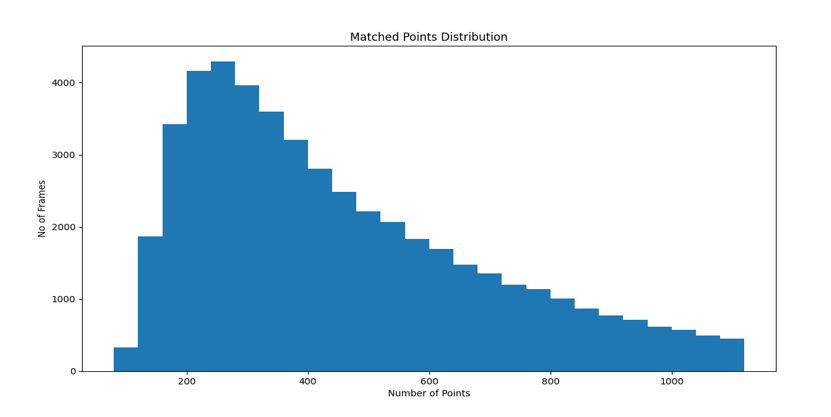
\includegraphics[ width=\textwidth]{figs/matched_points.png}
	\vspace{-0.5cm}
	\caption[Histogram of the number of matched points]{Histogram of the number of matched points. Vertical axis denotes the number of frames, with a given number of feature points detected.}
	\label{fig:ra:matched_points}
	\vspace{0.5cm}
\end{figure}

Furthermore, we calculated the average \gls{RMS} error obtained for a given number of matched points in a frame (see figure \ref{fig:ra:rms_error}), which showed that up to some optimal number, the \gls{RMS} error decreases with the number of matched points. However, beyond this point, it was observed that the \gls{RMS} error increases. A possible reason for this is the confusion caused by the large number of feature points (with similar features) detected very close to each other. When the number of detected features exceeds 1500, only the best 1500 features will be selected for the pose estimation mechanism, leaving the excess features unused. The saturation behaviour observed in the plot is a consequence of this.
\begin{figure}[h]
	\centering
	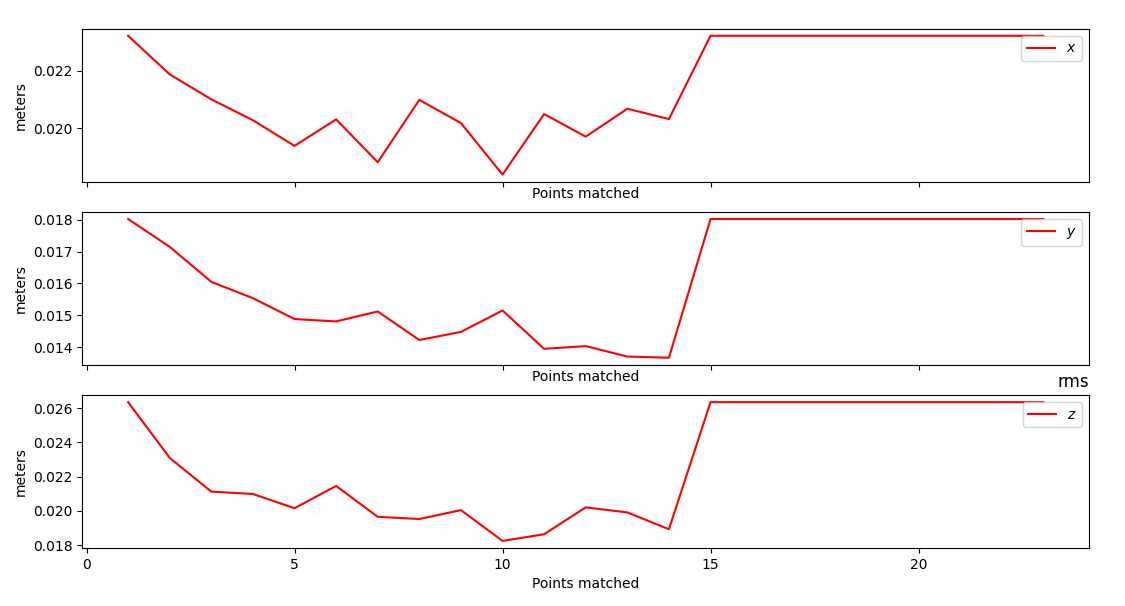
\includegraphics[ width=\textwidth]{figs/rms_error.png}
	\vspace{-0.5cm}
	\caption[Average \gls{RMS} error vs. the number of matched points]{Variation of average \gls{RMS} error, with the number of matched points (in hundreds)}
	\label{fig:ra:rms_error}
	\vspace{0.5cm}
\end{figure}


%%%%%%%%%%% ra end %%%%%%%%%%%%%%%%%%%%%%%








%%%%%%%%%%%%%%%% hi start %%%%%%%%%%%%%%%%%


\section{Lidar Odometry}
Following results were obtained using the \gls{KITTI} and \gls{KAIST} datasets. The frame of reference for the plots shown in the following discussion is the initial coordinate frame of the \gls{LiDAR} sensor, at the moment the vehicle started moving.

The \gls{LeGO-LOAM} algorithm creates a map of points through the map construction module and localize the vehicle within the map. Figure \ref{fig:ha:lidar_map} shows such a map and the predicted path of the vehicle in the map.
\begin{figure}[h]
	\centering
	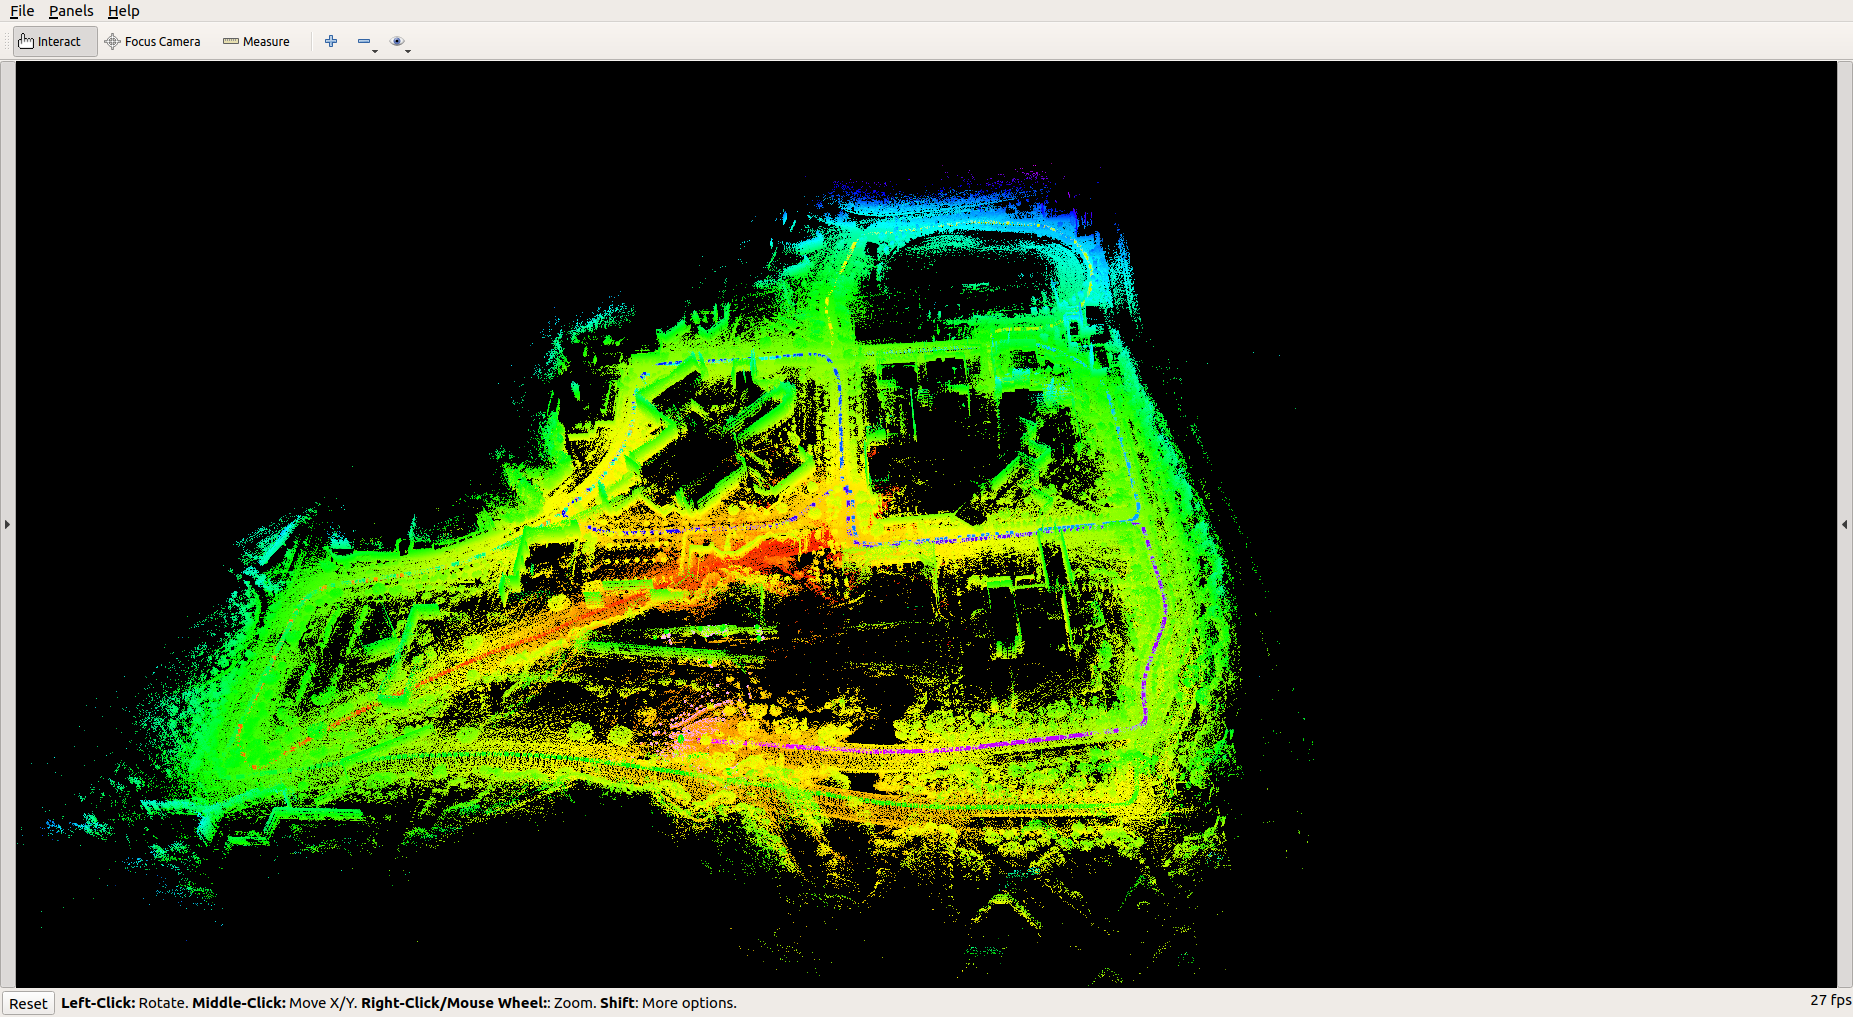
\includegraphics[width=\textwidth]{figs/rviz_lidar.png}
	\vspace{-0.2cm}
	\caption[\gls{LeGO-LOAM} generated \gls{SLAM} map using \gls{KAIST}dataset]{\gls{LeGO-LOAM} generated \gls{SLAM} map using \gls{KAIST}dataset. Coloured points are the \gls{LiDAR} point cloud points, based on their intensity level.}
	\label{fig:ha:lidar_map}
	\vspace{0.2cm}
\end{figure}

Figure \ref{fig:hi:xyz_error} shows the \gls{LeGO-LOAM} estimated position error in the directions of x, y and z, with the frame index and figure \ref{fig:hi:rpy_error} shows the error in roll, pitch and yaw with the frame index. It can be seen that, position error increase with time and reduces back to a lower value. The increase is caused by the error accumulation, while adding up the relative translations of the vehicle to obtain the overall position. The reduction in the error is a result of the system using loop closure global optimization method to optimize the path while building the map.

\begin{figure}[h]
	\centering
	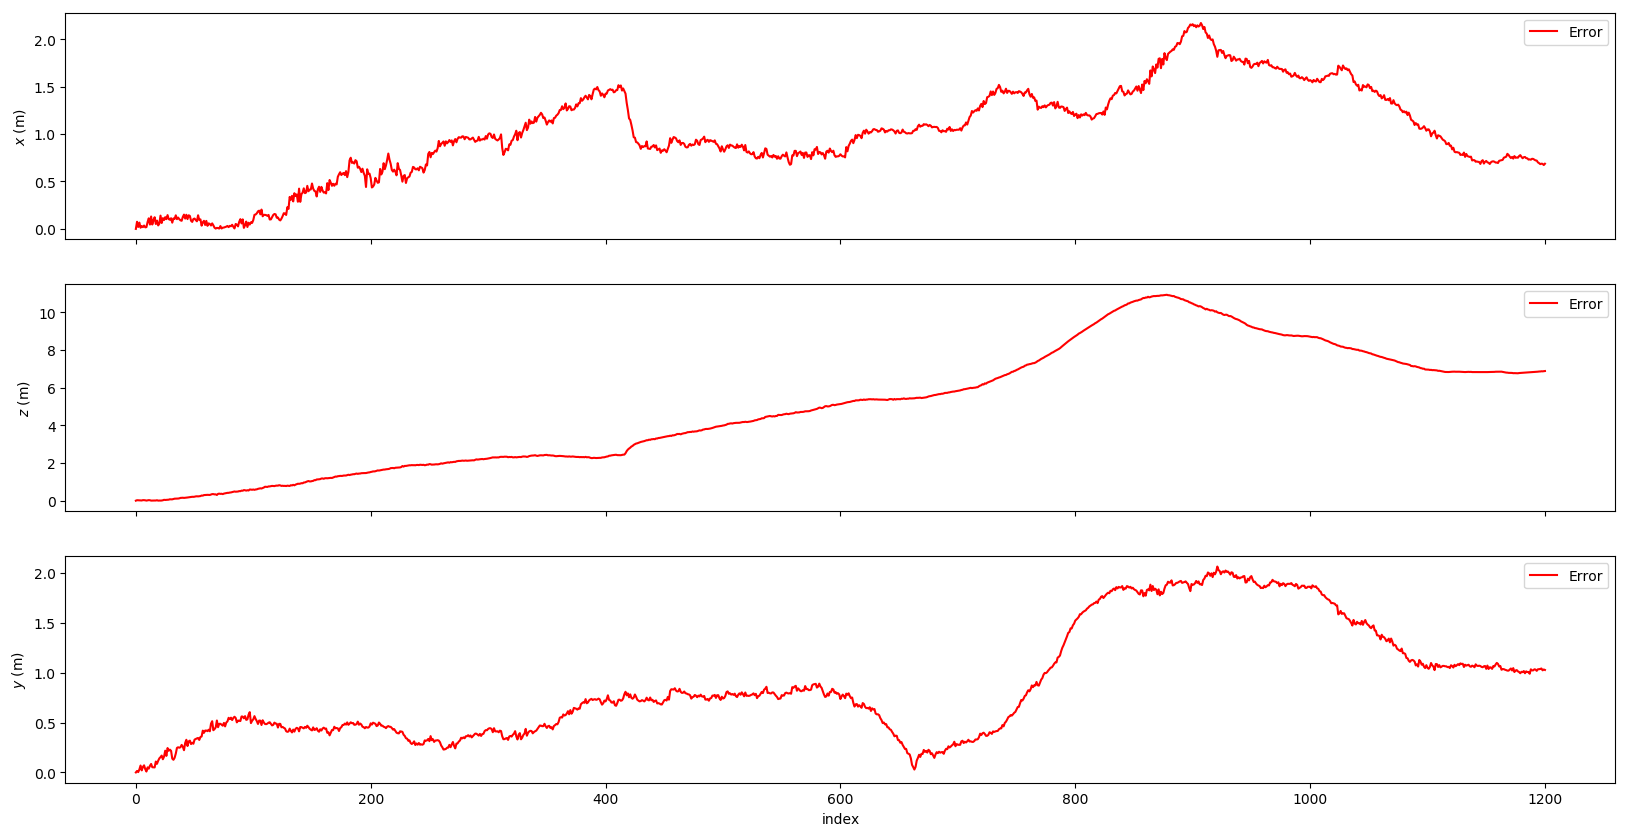
\includegraphics[ width=\textwidth]{figs/lidar_xyz_error.png}
	\vspace{-0.5cm}
	\caption{Error in x, y and z direction for \gls{KITTI} sequence 05}
	\label{fig:hi:xyz_error}
	\vspace{0.5cm}
\end{figure}

\begin{figure}[h]
	\centering
	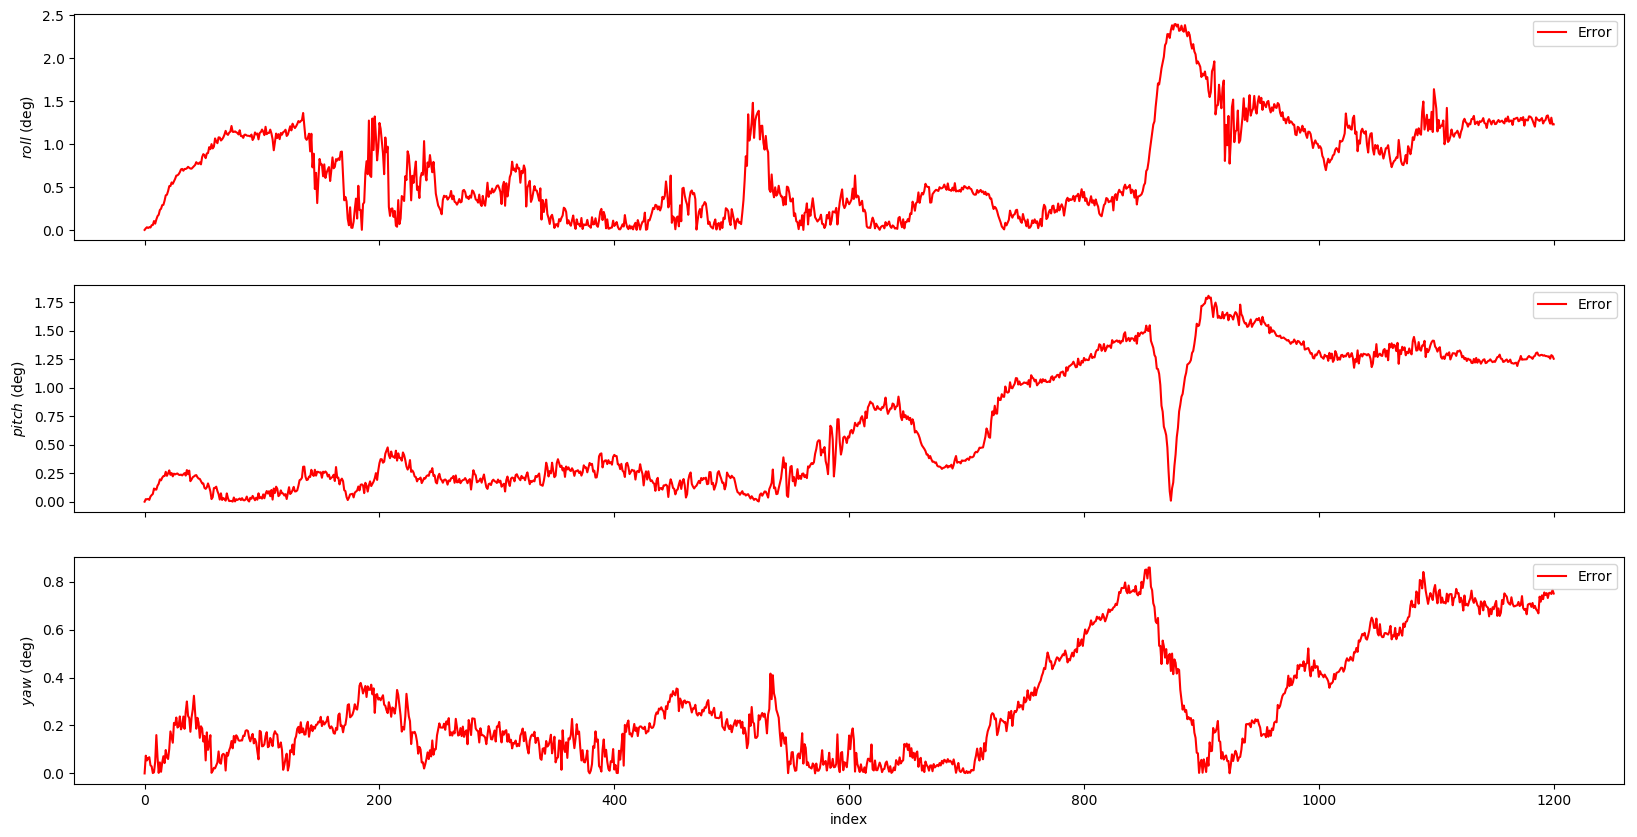
\includegraphics[ width=\textwidth]{figs/lidar_rpy_error.png}
	\vspace{-0.5cm}
	\caption{Error in roll, pitch and yaw for \gls{KITTI} sequence 05}
	\label{fig:hi:rpy_error}
	\vspace{0.5cm}
\end{figure}


%%%%%%%%%%%%%%%% hi end %%%%%%%%%%%%%%%%%%%%
  \chapter{Discussion and Conclusion}



  \singlespacing
  \addcontentsline{toc}{chapter}{References}
\renewcommand{\bibname}{\MakeUppercase{References}}
\bibliographystyle{IEEEtran}
\bibliography{thesis}
  % \chapter*{Appendix I}
\addcontentsline{toc}{chapter}{Appendix I}
\label{appendix:ESEKFMatrices}
% TODO: matrices of ES EKF


\end{document}
